\documentclass[a4paper]{article}
\usepackage{float}
\usepackage[ruled,vlined,linesnumbered,algo2e]{algorithm2e}
\usepackage{amsmath,amssymb}
\usepackage{makecell}
\usepackage{tikz}
\usepackage[margin=0.8in]{geometry}
%\usepackage{biblatex} %Imports biblatex package
%\addbibresource{NLA.bib}
\DeclareMathOperator*{\argmax}{arg\,max}
\DeclareMathOperator*{\argmin}{arg\,min}
\DeclareMathOperator*{\diag}{diag}
\DeclareMathOperator*{\trace}{trace}
\DeclareMathOperator*{\sign}{sign}

\newcommand*\circled[1]{\tikz[baseline=(char.base)]{
		\node[shape=circle,draw=red,inner sep=1pt] (char) {#1};}}
\newcommand{\mbf}[1]{\mathbf{#1}}
\setlength\parindent{0pt} %% Do not touch this
\usepackage{amsthm}
\newtheorem{lemma}{Lemma}
\newtheorem{theorem}{Theorem}
%% -----------------------------
%% TITLE
%% -----------------------------
\title{Homework: Regularization} %% Assignment Title
%% Change "\today" by another date manually
%% -----------------------------
%% -----------------------------

%% %%%%%%%%%%%%%%%%%%%%%%%%%
\newcommand\myemptypage{
	\null
	\thispagestyle{empty}
	\addtocounter{page}{-1}
	\newpage
}

\usepackage{fancyhdr}
\usepackage{listings}
%\usepackage{siunitx}
\usepackage{hyperref}
\usepackage{etoolbox,refcount}
\usepackage{multicol}
\usepackage{tabularx,colortbl}
\usepackage{lastpage}
\usepackage{pgfplots}
\pgfplotsset{compat = newest}
\usepackage{biblatex} %Imports biblatex package
%\addbibresource{NLA.bib}
\usepackage{diagbox}
\pagestyle{fancy}
\usepackage{caption}
\usepackage{subcaption}
\usepackage{mathtools}
\usepackage{cleveref}
\usepackage[bottom]{footmisc}
\usepackage{comment}
\usepackage{longtable}

\usepackage{lipsum} % just for dummy text- not needed for a longtable
\fancyhead[C]{}
\fancyhead[r]{}
%\renewcommand{\footrulewidth}{1pt}
\fancyfoot[L]{}
\fancyfoot[C]{}
\fancyfoot[R]{\thepage\ / \pageref*{LastPage}}

\begin{document}
	
	\begin{titlepage}
		
		\newcommand{\HRule}{\rule{\linewidth}{0.5mm}}  
		
		\begin{center}
			
			%\includegraphics[scale=0.3]{Documents/KUL_ENG.png}\\[1cm]
			\textsc{\LARGE Faculty of Engineering Science}\\[1.5cm] 
			
			
			\HRule \\[0.1cm]
			
			{\huge{ \bfseries Denoising and inpainting with wavelets}} 
			\vspace{5pt}
			{\\ \Large{\bfseries Wavelets with application in signal and Image processing}}
			\HRule \\[1cm]
			
			%\includegraphics[width=0.3\textwidth]{images1/INEOS.png}\\
			\vspace*{0.1cm}
			
			\begin{minipage}{0.4\textwidth}
				\textit{Auteur}
				\begin{flushleft} \large
					\begin{enumerate}
						\item[] \textsc{Thakur} Arnav\\
                        \item[] \textsc{Mohamed Yassin} Arman\\

						
					\end{enumerate} 
				\end{flushleft}
			\end{minipage}\\[1cm]
			\begin{minipage}{0.4\textwidth}
				\textit{Professors}
				\begin{flushleft}
					\begin{enumerate}
						\item[] Prof. Daan Huybrechs\\
					\end{enumerate} 
				\end{flushleft}
			\end{minipage}\\
			
			\vspace*{1.5cm}
			
			
\includegraphics[width=0.5\textwidth]{Images/KUL_Eng_logo.png}\\
			{\Large{Academic year 2023 - 2024}}
			
		\end{center}
	\end{titlepage}
	
	\newpage
	
	\tableofcontents
	
	\newpage

    \section{Wavelet-based denoising}
 
	\subsection{A univariate functions with noise} \label{subsec:UniVariate}

    \subsubsection{Question 2.1}

	Consider the function:
    \begin{equation} \label{eq:func}
	f(x) = (2+\cos{(x)}) |x| \sign{(x-1)}
	\end{equation}
    Function sampled in a set of $N=1000$ points in the interval $[-2,2]$
    \begin{align*}
    	f_j = f(x_j) && x_j = -2 + 4\frac{j-1}{N-1}, \quad j=1,\ldots,N
    \end{align*}
    
    We compute the wavelet transform of the vector $f = \{f_j\}_{j=1}^N$ using the Daubechies 2 wavelet of 5 levels deep. boundary conditions used is: Symmetrization (half-point). These same parameters are used for the rest of \cref{subsec:UniVariate}. The wavelet transform is computed using matlab \texttt{wavedec} and it's inverse using \texttt{waverec}. One of former's outputs is an array of wavelet coefficients $x$, this array is later thresholded for the propose of denoising. The signal can then be reconstructed using \texttt{waverec}, one whose arguments is $x$.
    
    \begin{figure}[H]
	\centering
	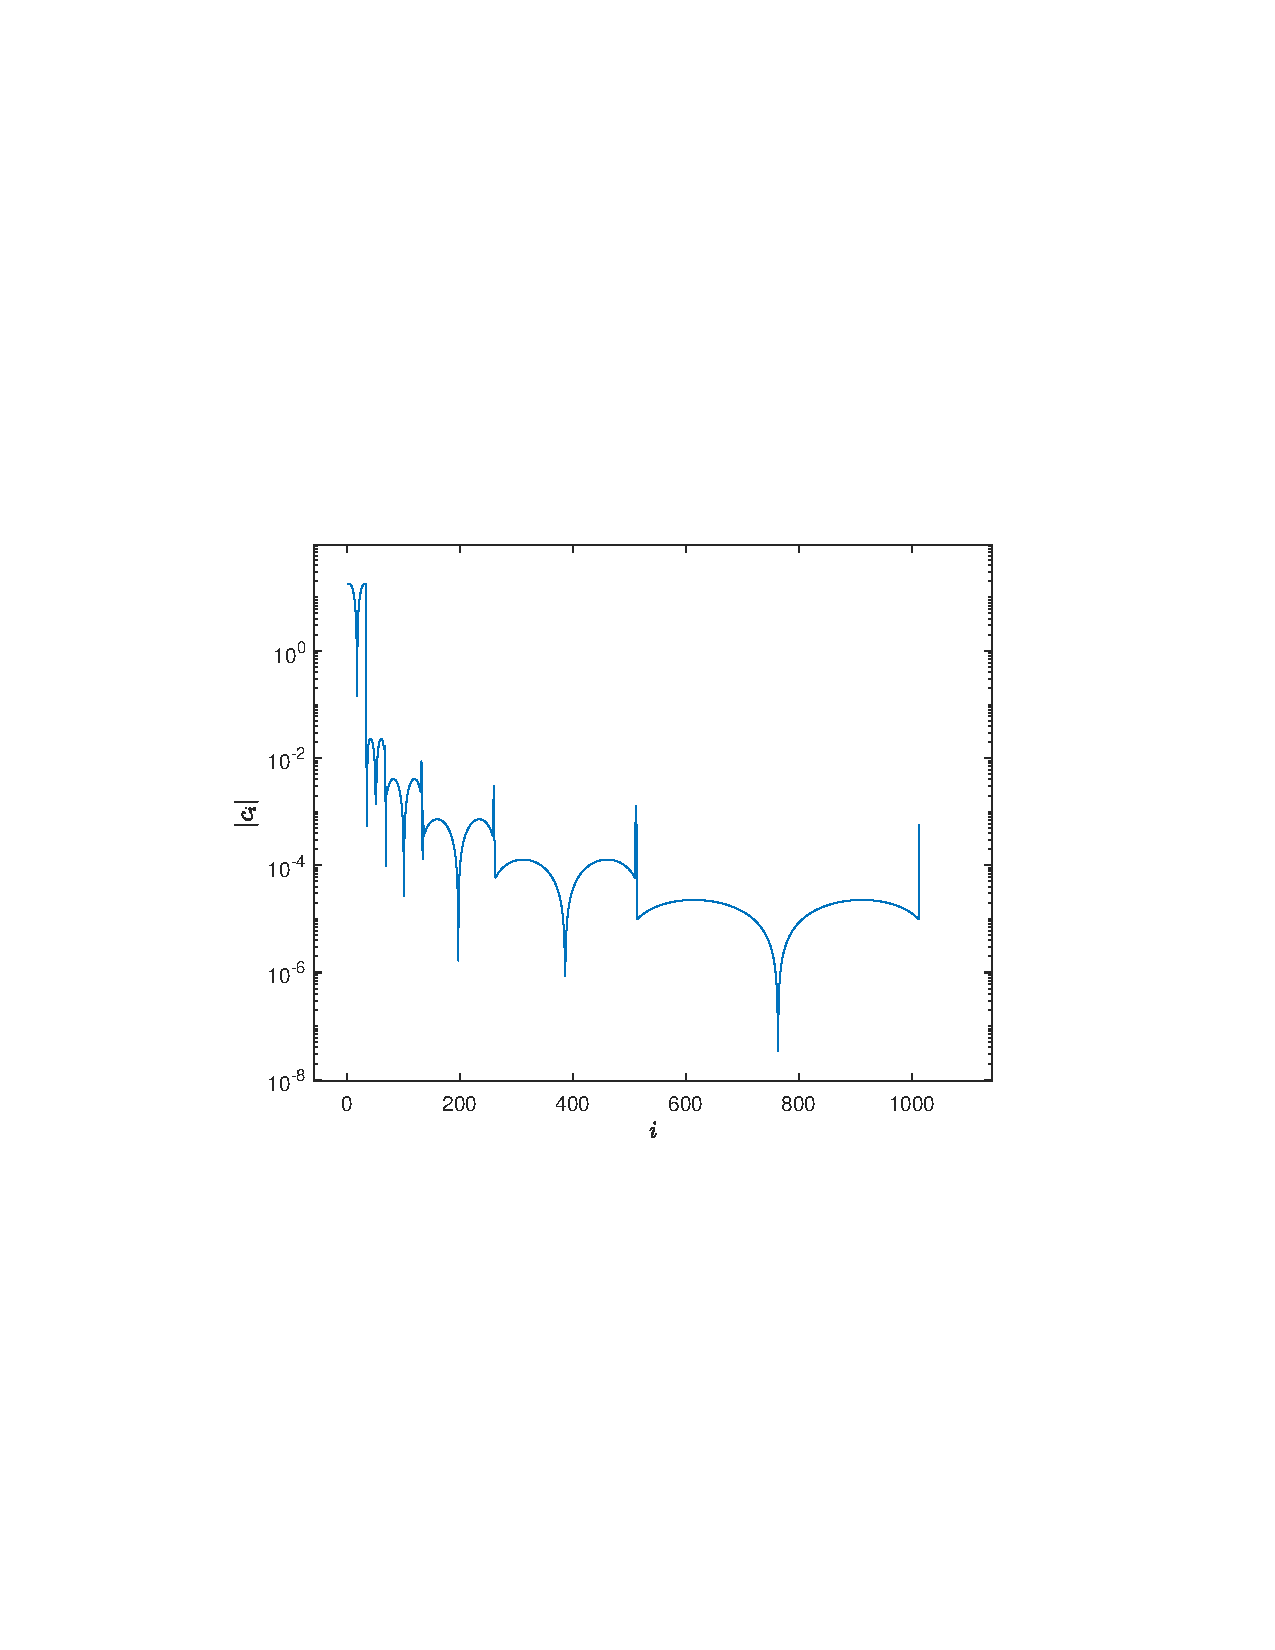
\includegraphics[trim={3.5cm 8cm 4cm 9cm},clip,width=0.7\textwidth]{Images/Coefficents.pdf}
	\caption{Coefficients of Wavelet transform (5 levels deep, using the Daubechies 2, $N=1000$ sample points, between $[-2,2]$. DWT Extension Mode: Symmetrization (half-point)}
	\label{fig:Coeff}
    \end{figure}

    We can see in \footnote{To recreate \cref{fig:Coeff,fig:Delta=0,fig:Delta=0.1,fig:HardSoft,fig:OptiDelta} run \texttt{ex2point1.m}} \cref{fig:Coeff}, that the size of the coefficients decreases as $i$ increases. The meaning of this is that the coefficients of small size are of less importance to the reconstruction of the signal, and thus removing them will disproportionally remove noise.

    \subsubsection{Task 2.2} \label{subsubsec:thresholding}

	Noise is added to the signal $\tilde{f_i} = f_i + \epsilon \mathcal{U}(0,1)$ ($\hat{f}$ is the reconstructed $\tilde{f}$). We chose $\epsilon = \texttt{1e-1}$. \\
	Both hard thresholding:
	\begin{equation*}
			t_\delta = \begin{cases}
				0, \quad |x| < \delta\\
				x, \quad |x| \ge 0
		\end{cases}
	\end{equation*}
	And soft thresholding
	\begin{equation*}
			t_\delta = \begin{cases}
			0, \quad |x| < \delta\\
			\sign{(x)} (|x|-\delta), \quad |x| \ge 0
	\end{cases}
	\end{equation*}
	are going to be tested. $x$ are the wavelet coefficients.\\
	First let us choose $\delta = 0$, the results are in \cref{fig:Delta=0}. We can see in \cref{sub:ErrCoeffD=0}, that the highest error is in the first few coefficients. Which makes sense since we are in some sense moving the mean of the function $f$ by adding a value sampled from the uniform distribution, $\rightarrow$ lower frequencies should be more effected. The total error $E = \|f-\hat{f}\|_2 = 1.805$.\\
	
	Now let us set $\delta = \texttt{1e-1}$, the resulting figures are \cref{fig:Delta=0.1}. 3.35\% of the wavelet coefficients were set to 0, for both types of thresholding. \\
	For hard thresholding, $E = 1.5643$, which is indeed lower then the previous one. This seems manly due to the fact that $\hat{f}$ is smoother then $\tilde{f}$, see \cref{sub:ErrorD=0.1}. \\
	If knowledge of the mean of the noise is available, we can come put a better reconstruction of $f$ by $\hat{f}-mean(noise)$, in fact this is what will be done for the rest of \cref{subsec:UniVariate}, the resulting $E = 0.1982$, see \cref{sub:Delta=0.1Better}. In \cref{sub:Delta=0.1BetterSoft}, we can see the error when using soft thresholding, $E = 0.61$.

\begin{figure}[H]
	\centering
	\begin{subfigure}{0.49\textwidth}
	\centering
	%trim={<left> <lower> <right> <upper>}
	%\includegraphics[trim={4cm 8cm 4cm 8cm},clip,width=.49\textwidth]{Images/LQG_weighted4.pdf}
	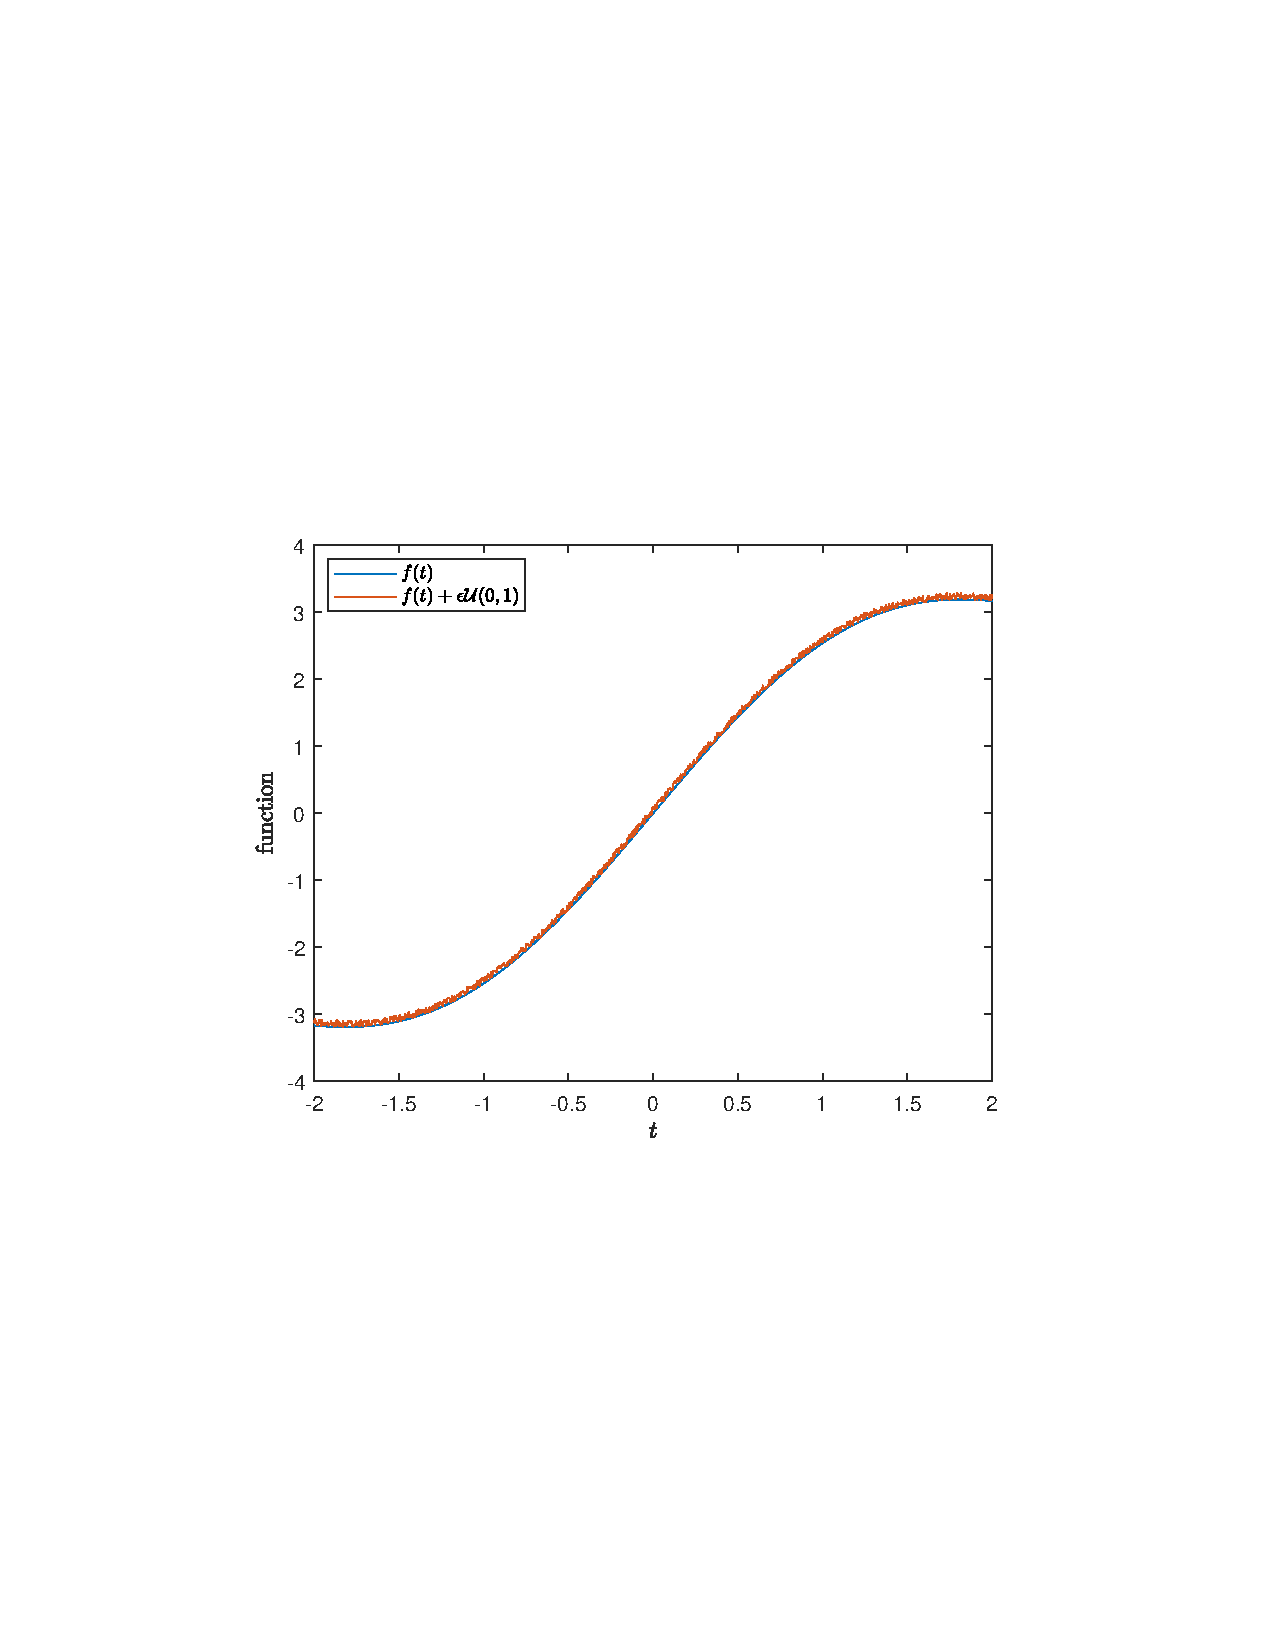
\includegraphics[trim={4cm 8cm 4cm 8cm},clip,width=1\textwidth]{Images/FuncNoise.pdf}
	\caption{Plot of function \cref{eq:func}, and it's noisy counterpart}
	\label{sub:FuncNoiseD=0}
\end{subfigure}
	\begin{subfigure}{0.49\textwidth}
		\centering
		%trim={<left> <lower> <right> <upper>}
		%\includegraphics[trim={4cm 8cm 4cm 8cm},clip,width=.49\textwidth]{Images/LQG_weighted4.pdf}
		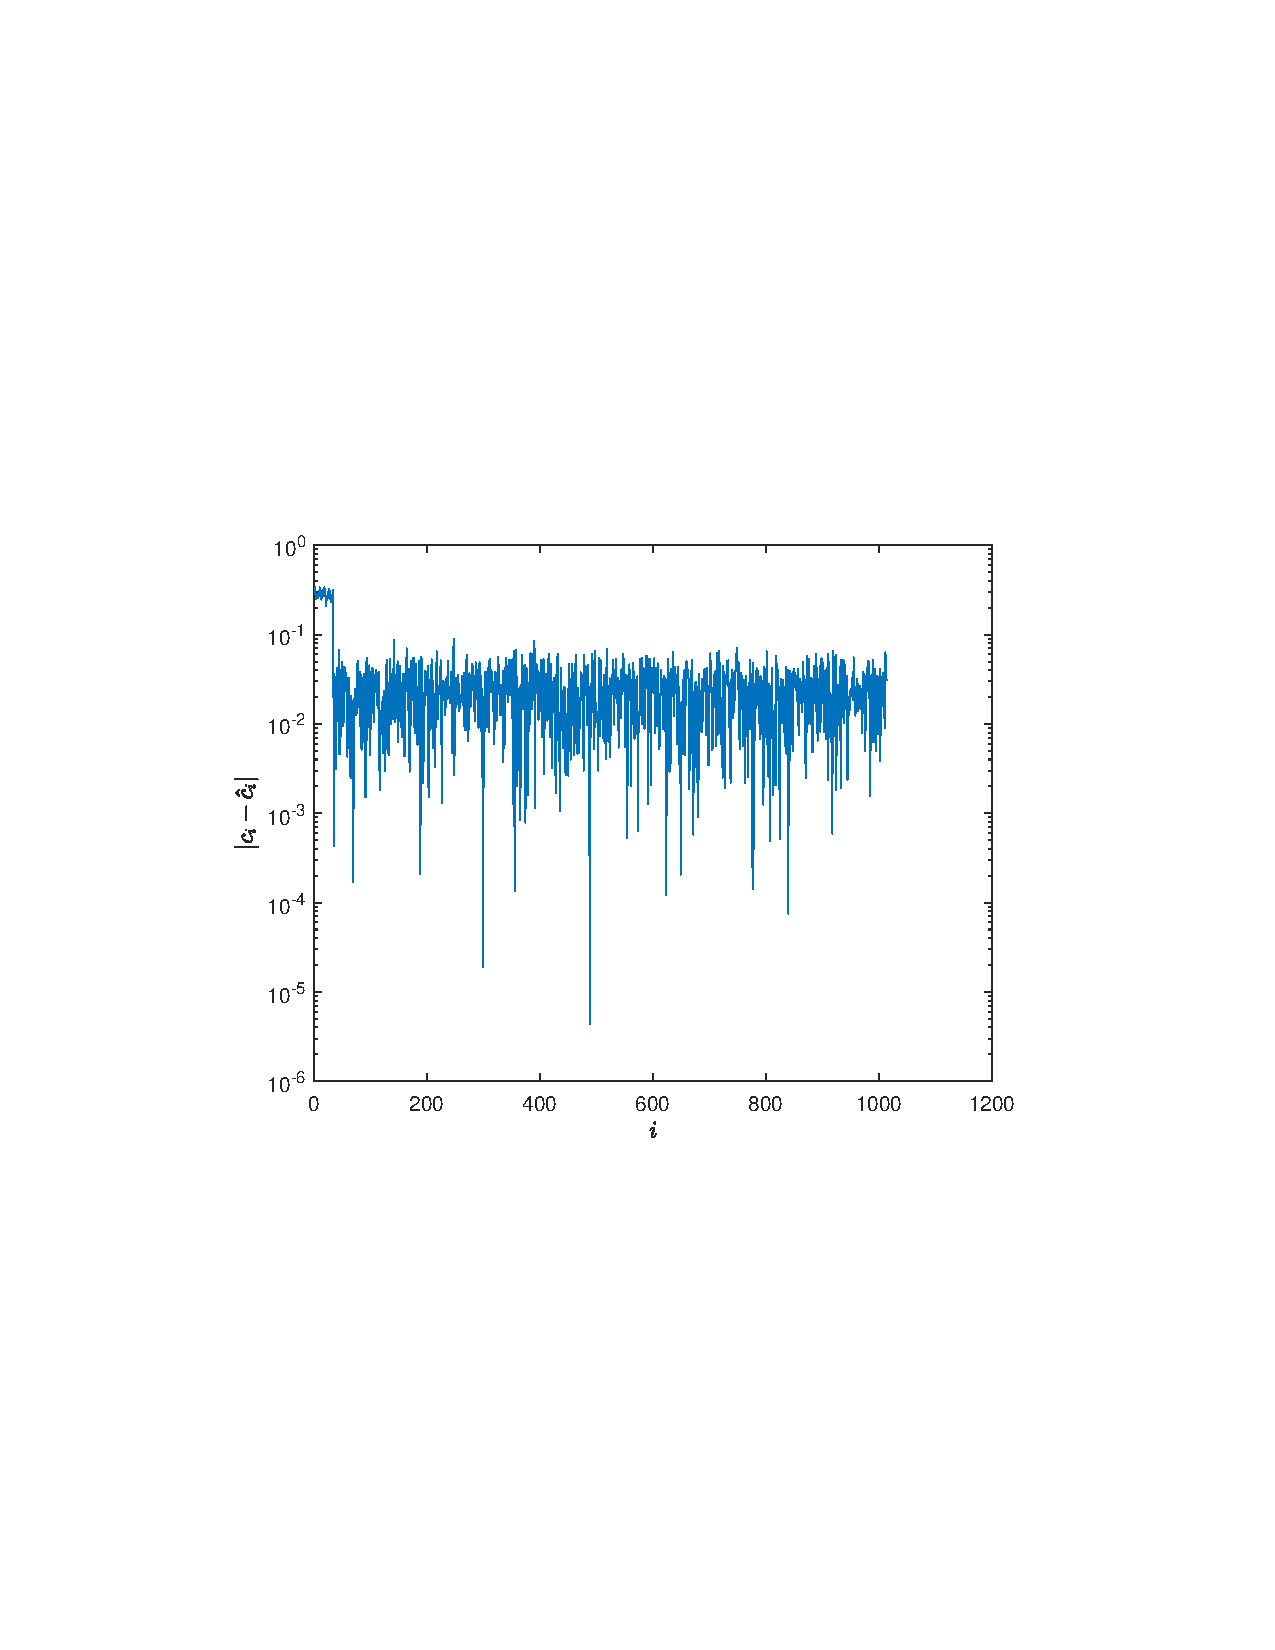
\includegraphics[trim={4cm 8cm 4cm 8cm},clip,width=1\textwidth]{Images/CoeffDelta=0.pdf}
		\caption{The error between the real coefficients and noisy ones}
		\label{sub:ErrCoeffD=0}
	\end{subfigure}
	\begin{subfigure}{0.49\textwidth}
		\centering
		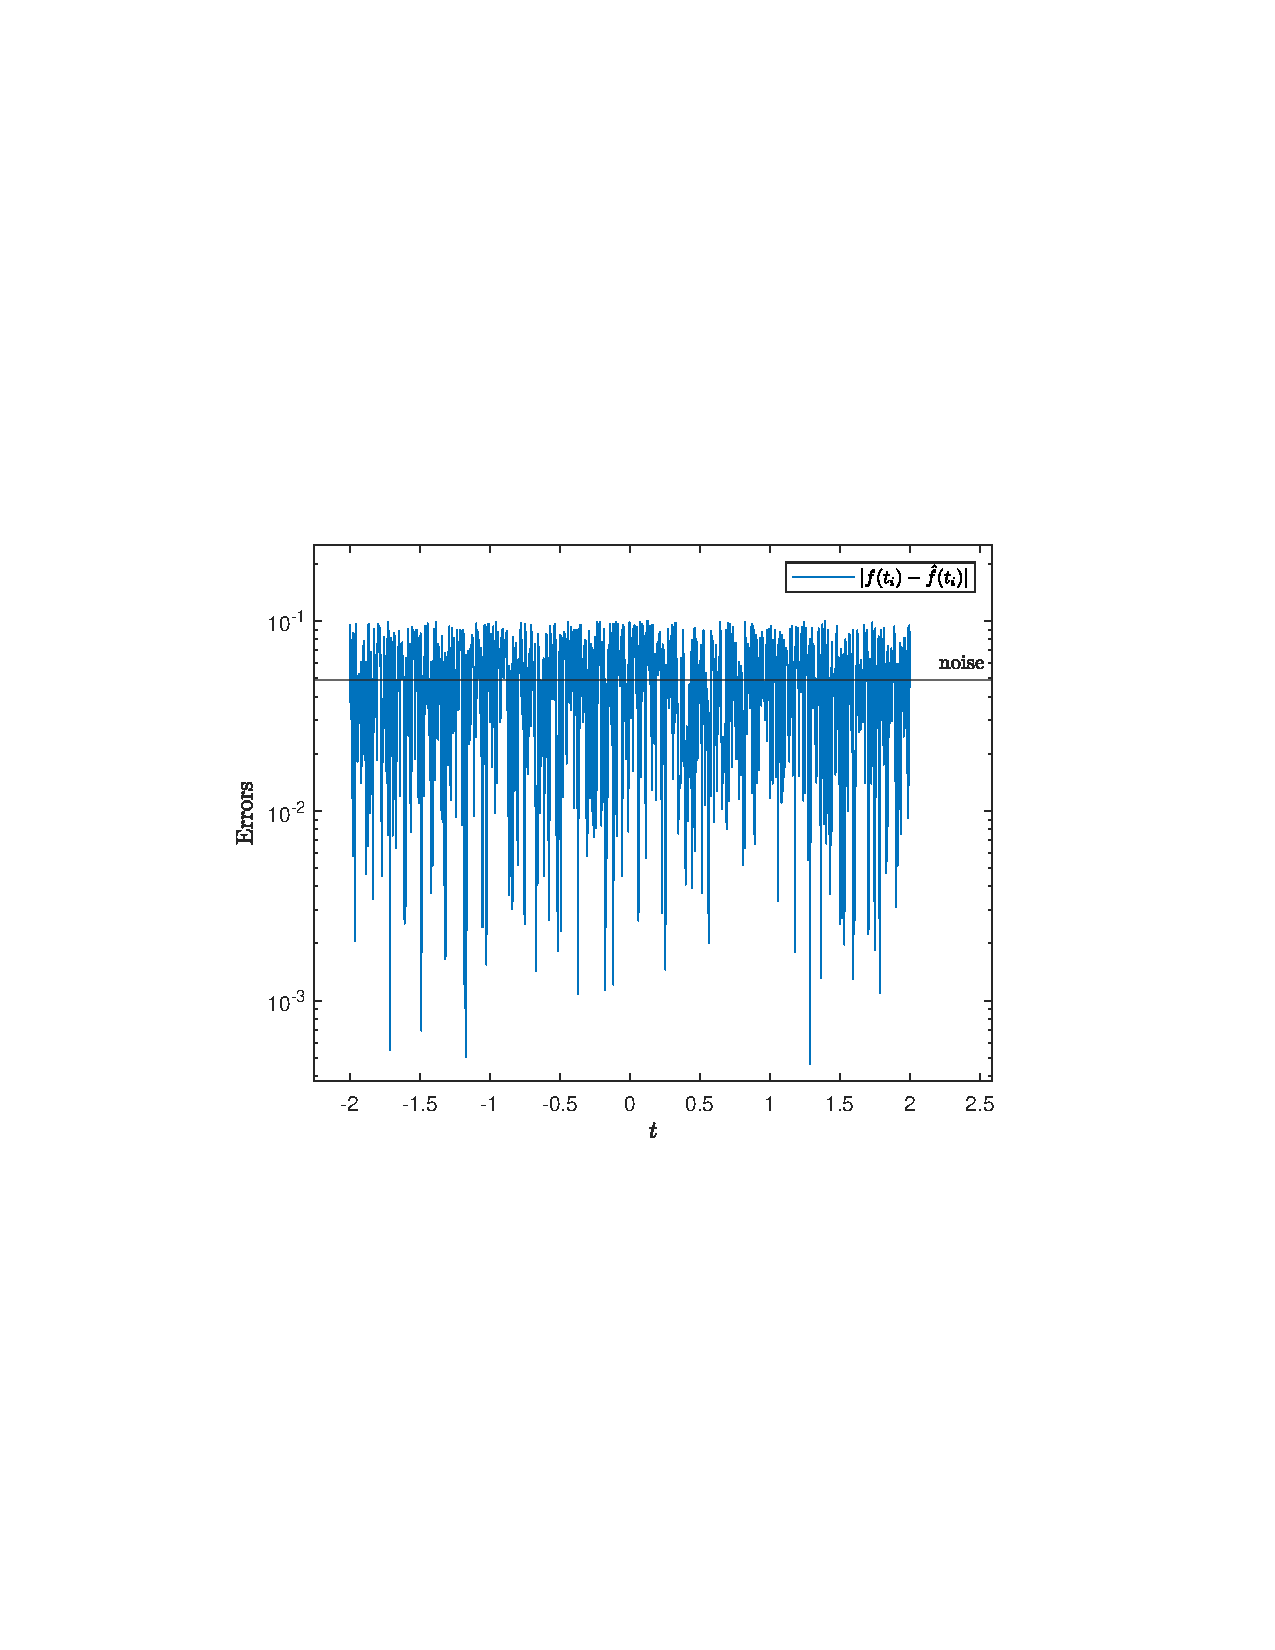
\includegraphics[trim={4cm 8cm 4cm 8cm},clip,width=1\textwidth]{Images/Delta=0.pdf}
		\caption{The error between real signal and noisy one}
		\label{sub:ErrorD=0}
	\end{subfigure}
	\caption{Plots for $\delta = 0$, black line is mean of noise. For hard thresholding}
	\label{fig:Delta=0}
\end{figure}

\begin{figure}[H]
	\centering
	\begin{subfigure}{0.49\textwidth}
		\centering
		%trim={<left> <lower> <right> <upper>}
		%\includegraphics[trim={4cm 8cm 4cm 8cm},clip,width=.49\textwidth]{Images/LQG_weighted4.pdf}
		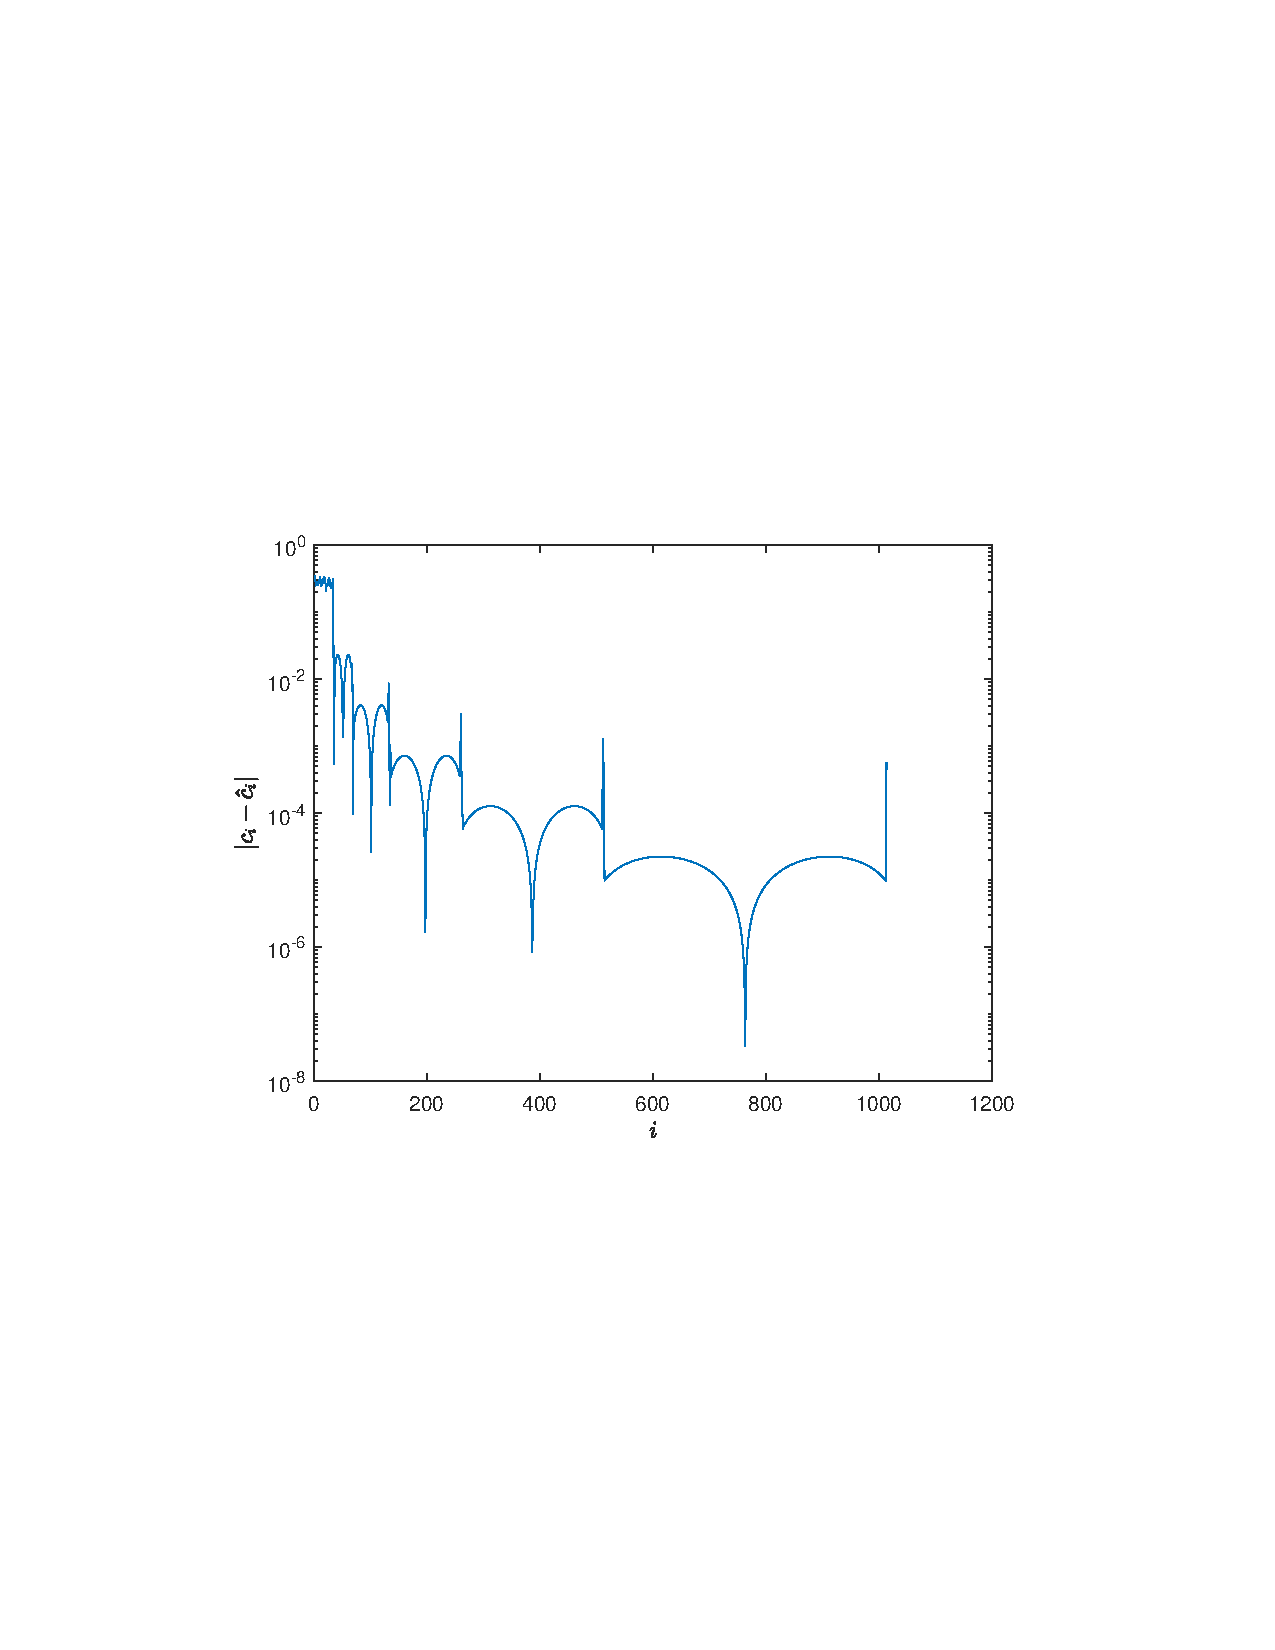
\includegraphics[trim={4cm 8cm 4cm 8cm},clip,width=1\textwidth]{Images/CoeffDelta=0.1.pdf}
		\caption{The error between the real coefficients and reconstructed ones}
		\label{sub:ErrCoeffD=0.1}
	\end{subfigure}
	\begin{subfigure}{0.49\textwidth}
		\centering
		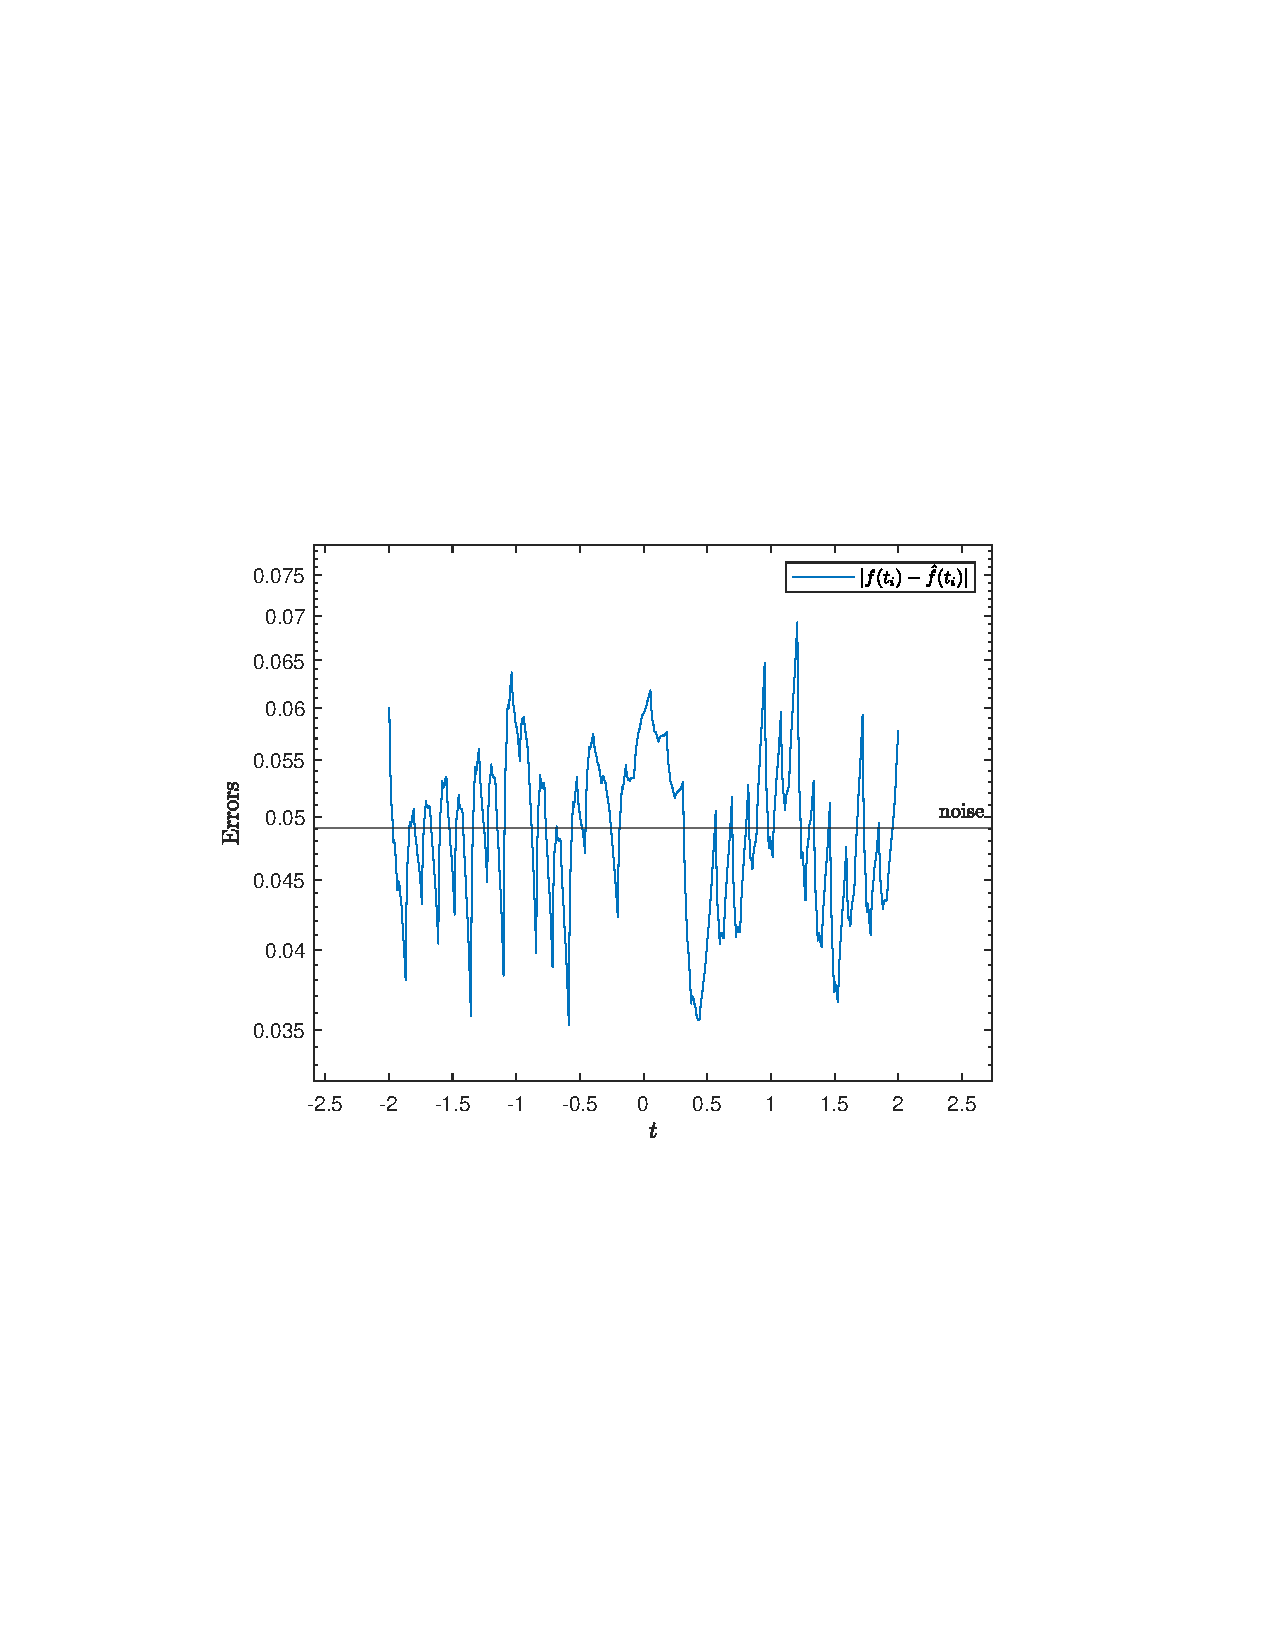
\includegraphics[trim={3.5cm 8cm 4cm 8cm},clip,width=1\textwidth]{Images/Delta=0.1.pdf}
		\caption{The error between real signal and reconstructed one}
		\label{sub:ErrorD=0.1}
	\end{subfigure}
	\caption{Plots for $\delta = 0.1$, black line is mean of noise. For hard thresholding}
	\label{fig:Delta=0.1}
\end{figure}

    \begin{figure}[H]
	\begin{subfigure}{0.49\textwidth}
	\centering
	\centering
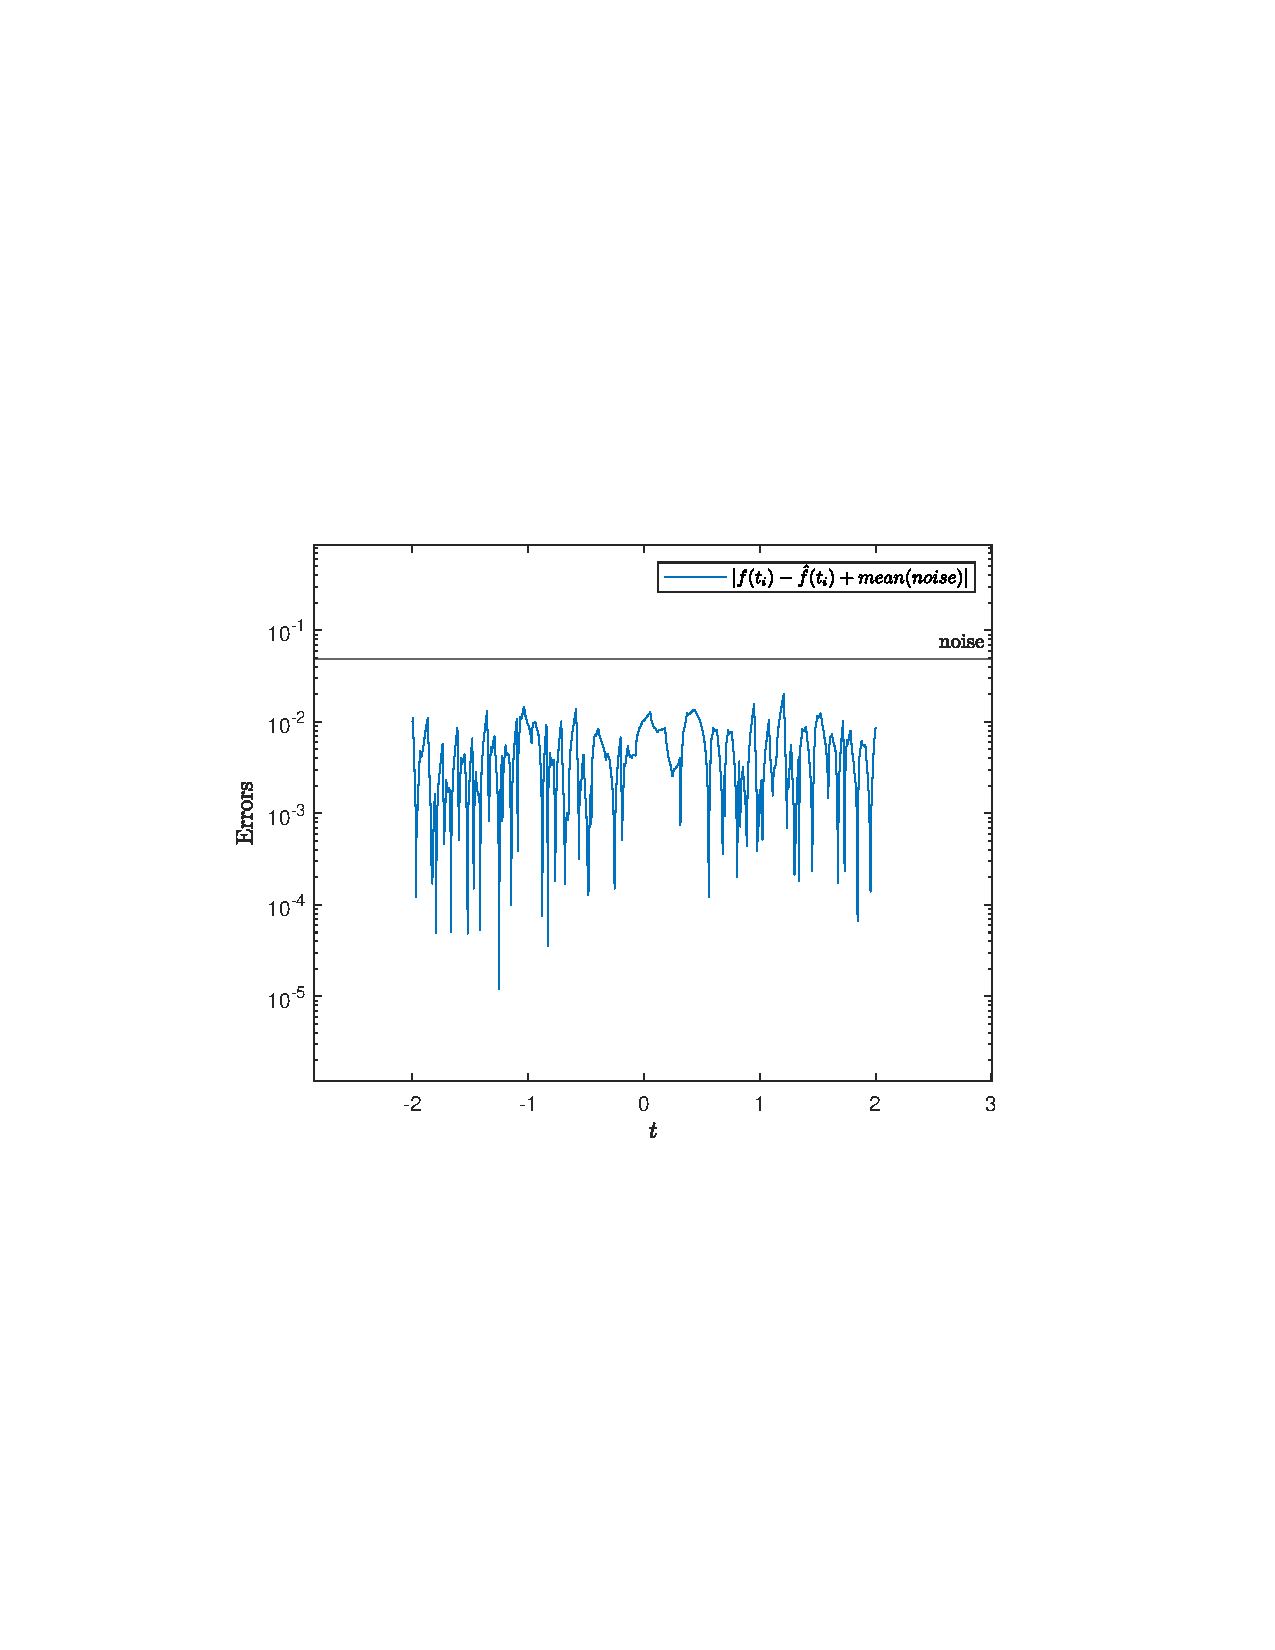
\includegraphics[trim={3.5cm 8cm 4cm 9cm},clip,width=1\textwidth]{Images/Delta=0.1Better.pdf}
\caption{The error between real signal and reconstructed one, black line is mean of noise. For hard thresholding}
\label{sub:Delta=0.1Better}
\end{subfigure}
\begin{subfigure}{0.49\textwidth}
	\centering
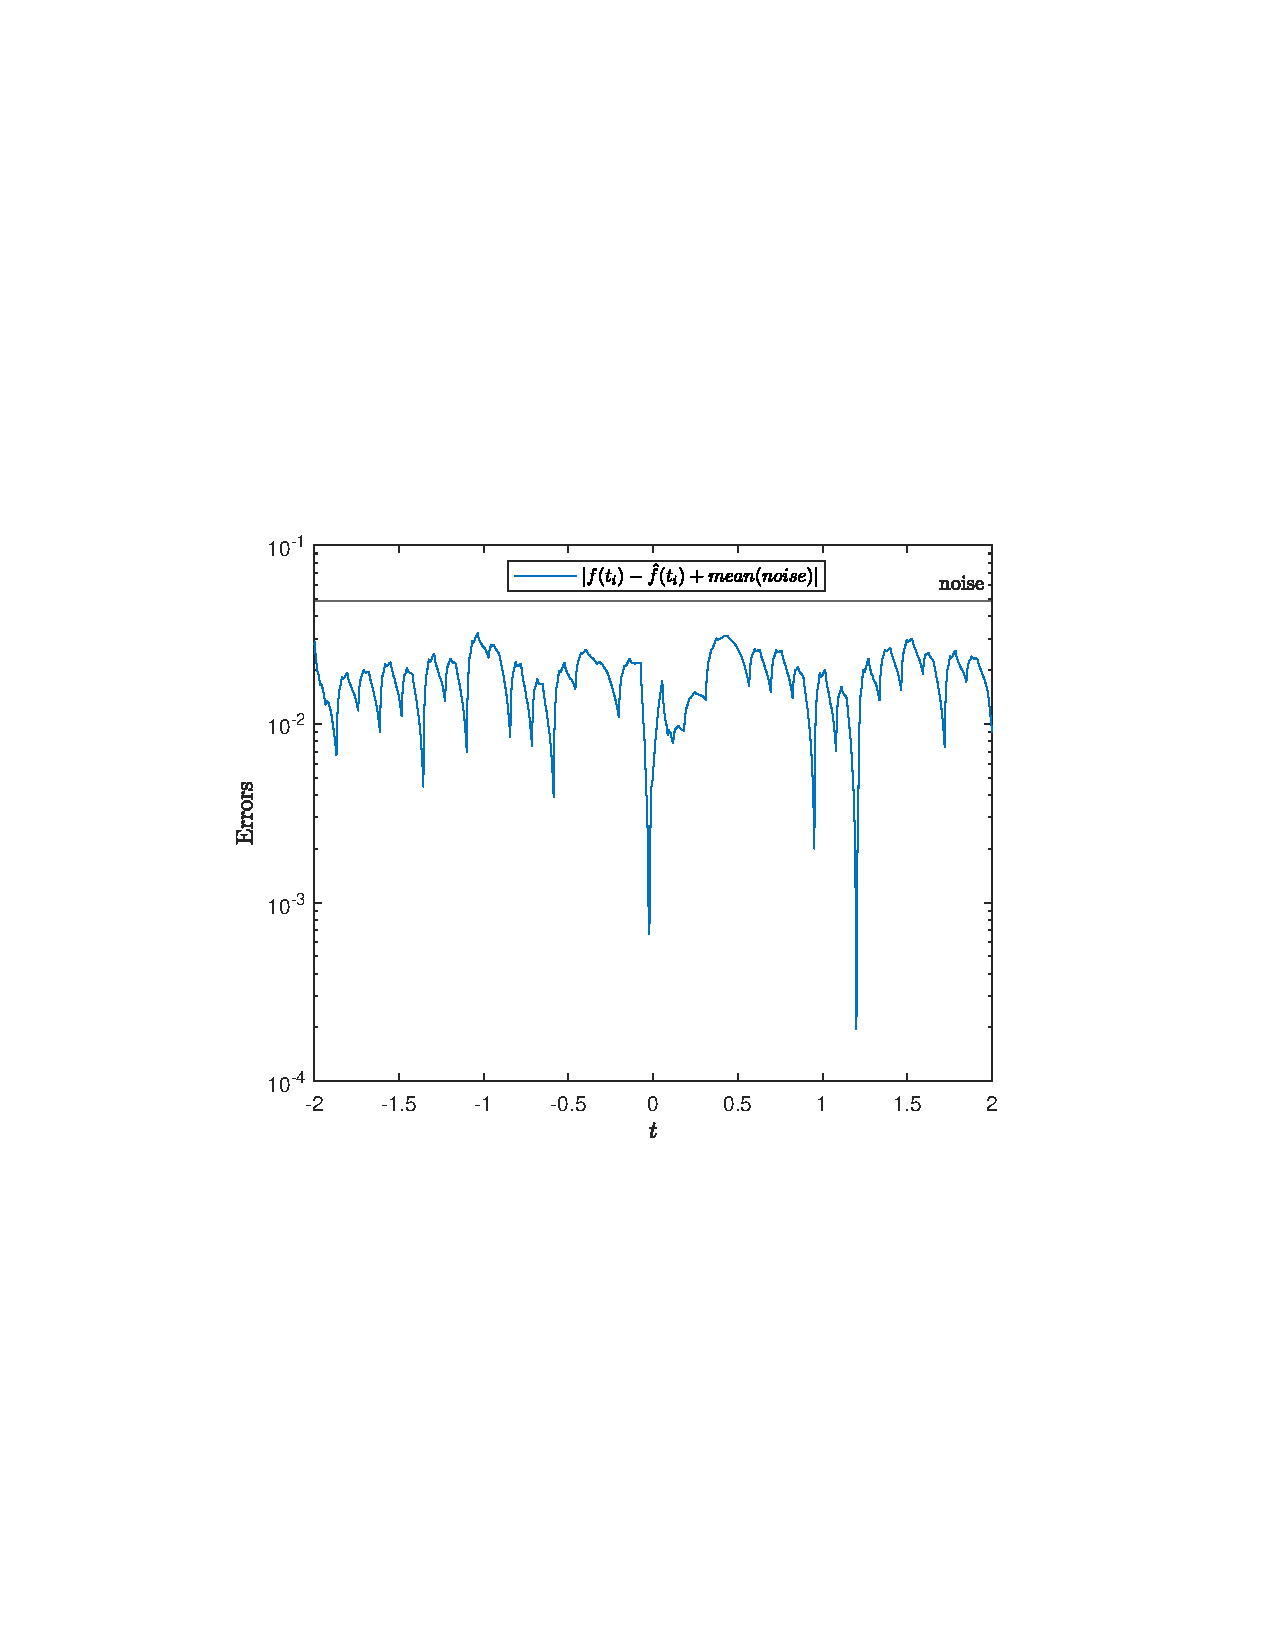
\includegraphics[trim={3.5cm 8cm 4cm 9cm},clip,width=1\textwidth]{Images/Delta=0.1Soft.pdf}
\caption{The error between real signal and reconstructed one, black line is mean of noise. For soft thresholding}
\label{sub:Delta=0.1BetterSoft}
\end{subfigure}
\caption{}
\label{fig:HardSoft}
\end{figure}


    \subsubsection{Question 2.3}

	Now let us try to find the best parameter $\delta$ in order to minimize the noise. This will be done by simply checking MSE between the real and filtered coefficients $\sum_{i} (x_i - \hat{x}_i)^2$, for 101 different equidistant $\delta$'s in $[\texttt{1e-10},\texttt{1e0}]$. The results are shown in \cref{fig:OptiDelta}, the best delta according to MSE is 
	\begin{itemize}
		\item Hard threshold: $\delta = 0.501$ with an MSE=0.0026
		\item Soft threshold: $\delta = 0.0398$ with an MSE=0.0028
	\end{itemize}
	The reconstructed functions do have visibly less error then the noisy one \cref{sub:FuncNoiseD=0}.\\
	For hard thresholding, the error is especially noticeable for $x = 0$ (\cref{sub:BestDelta,sub:BestDeltaFunc}), probably due to the fact that $f$ is not differentiable due to $|x|$, and because of the very discontinuous nature of the thresholding this results in more error. For $x = 1$, we can also see a slight bump in error due the discontinuation of the $\sign$ function.\\
	For soft thresholding it would seem that the error is higher over the whole domain but lower in $x=0$, due to the fact that it is less discontinuous then hard thresholding. (\cref{sub:BestDeltaSoft,sub:BestDeltaSoftFunc}) \\
	
	It would seem that hard thresholding is overall smoother then soft except for $x=0$. 

    \begin{figure}[H]
	\begin{subfigure}{0.49\textwidth}
	\centering
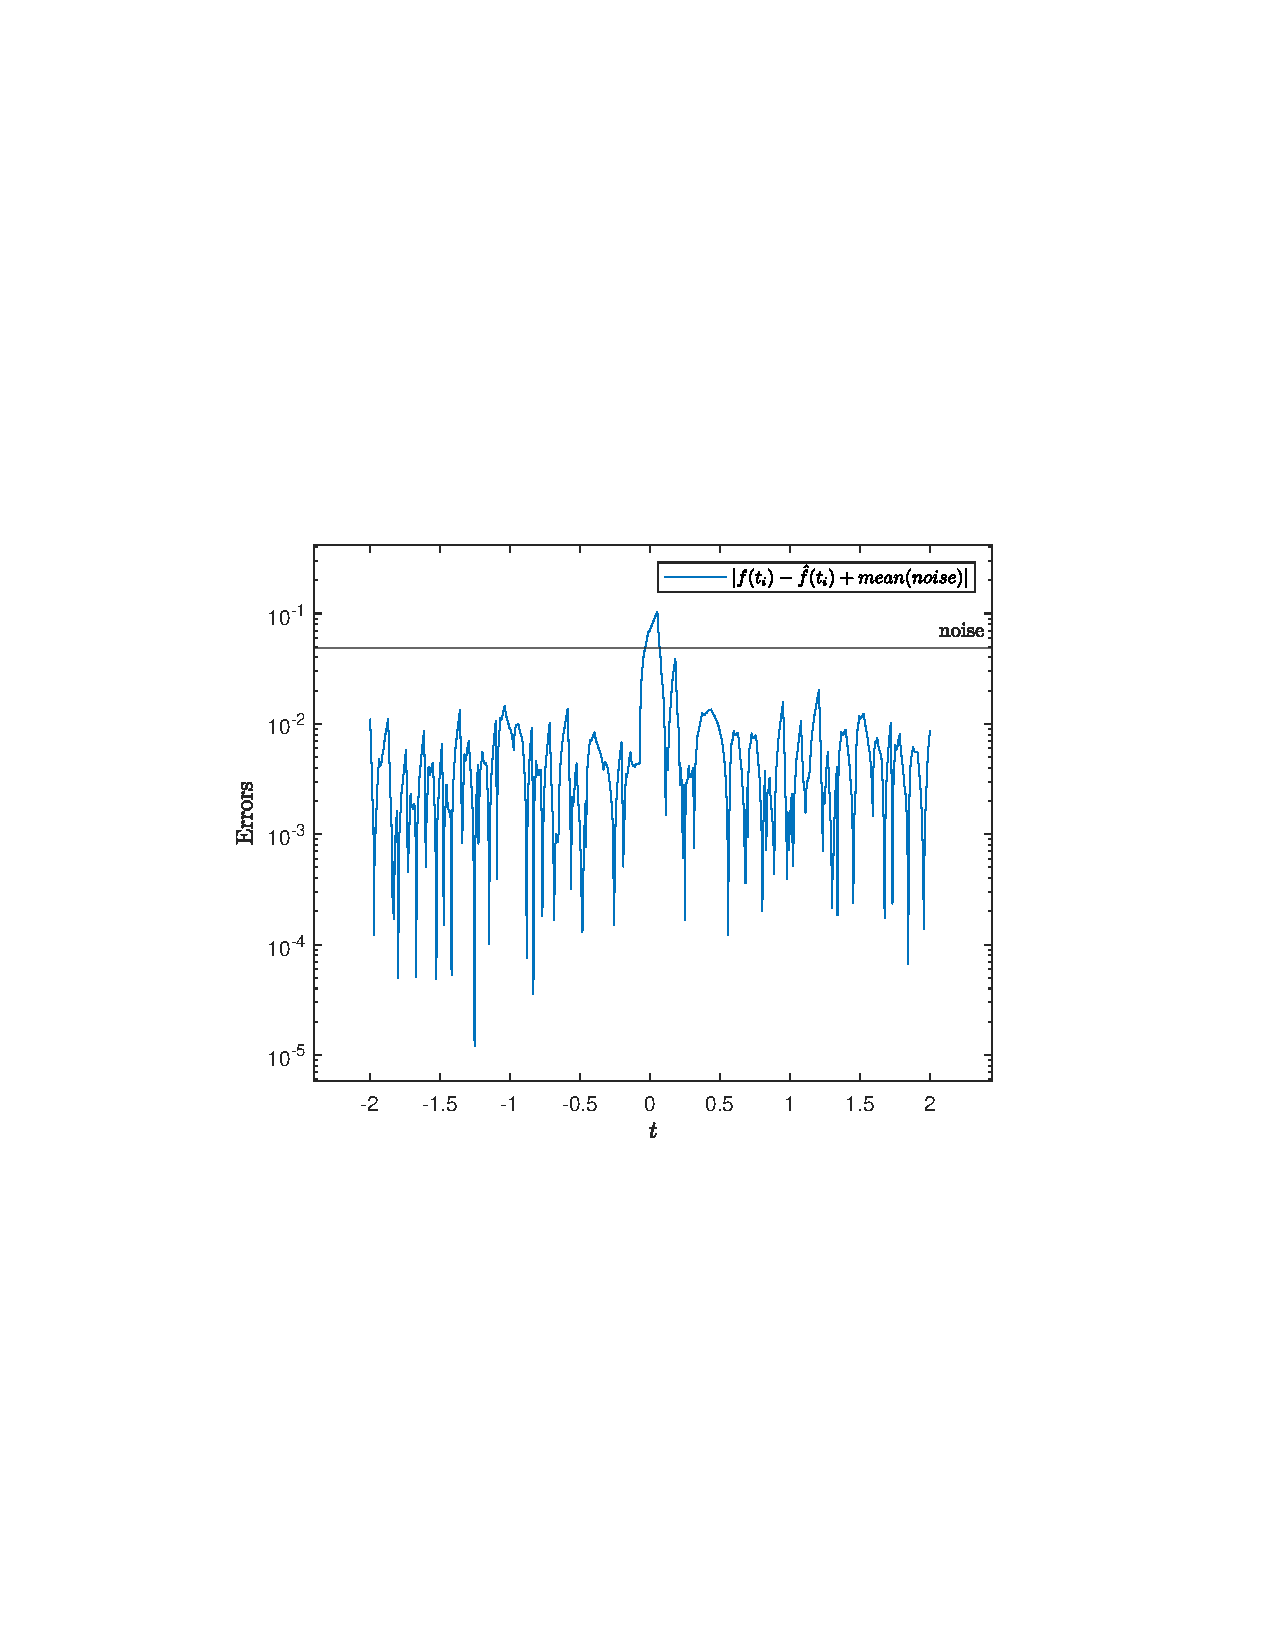
\includegraphics[trim={3.5cm 8cm 4cm 9cm},clip,width=1\textwidth]{Images/DeltaOpti.pdf}
\caption{The error between real signal and reconstructed one, black line is mean of noise. $\delta = 0.501$. For Hard thresholding}
\label{sub:BestDelta}
\end{subfigure}
\begin{subfigure}{0.49\textwidth}
	\centering
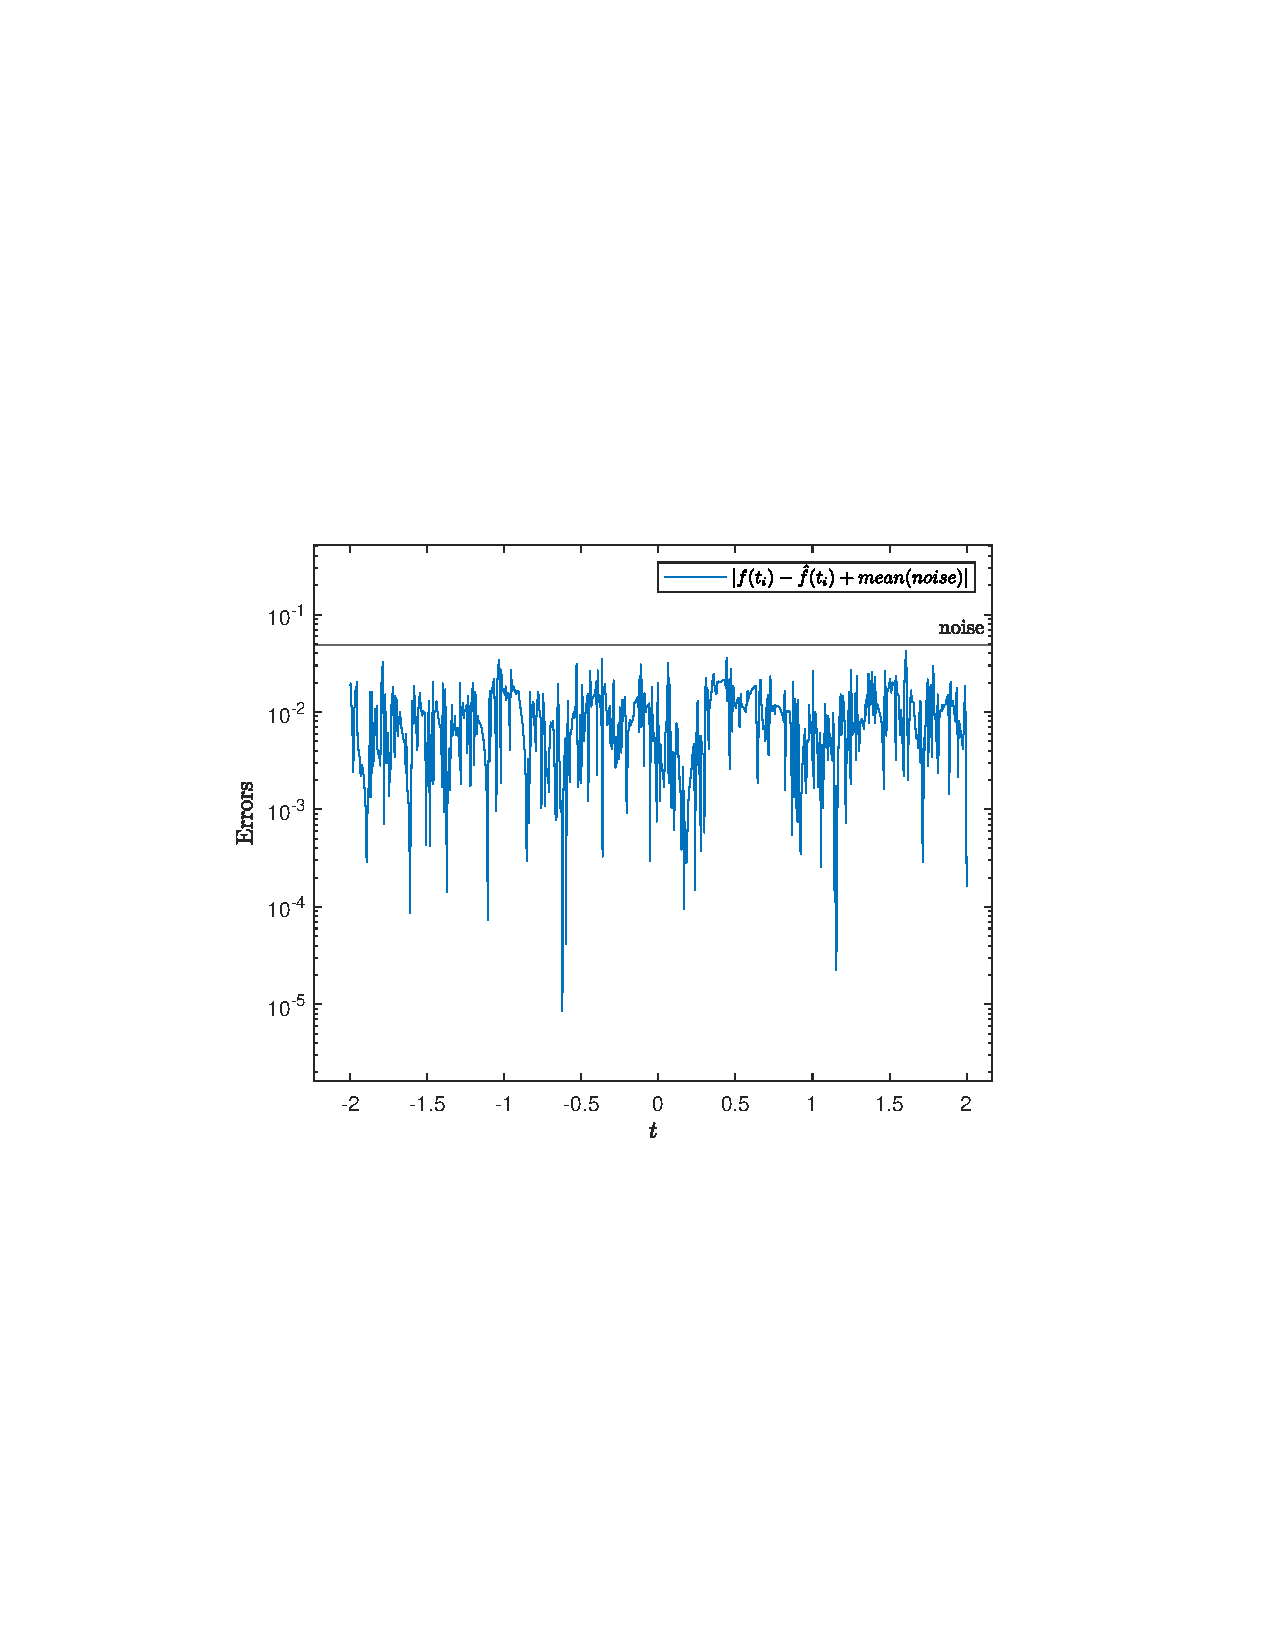
\includegraphics[trim={3.5cm 8cm 4cm 9cm},clip,width=1\textwidth]{Images/DeltaOptiSoft.pdf}
\caption{The error between real signal and reconstructed one, black line is mean of noise.$\delta = 0.0398$. For soft threasholding}
\label{sub:BestDeltaSoft}
\end{subfigure}
	\begin{subfigure}{0.49\textwidth}
	\centering
	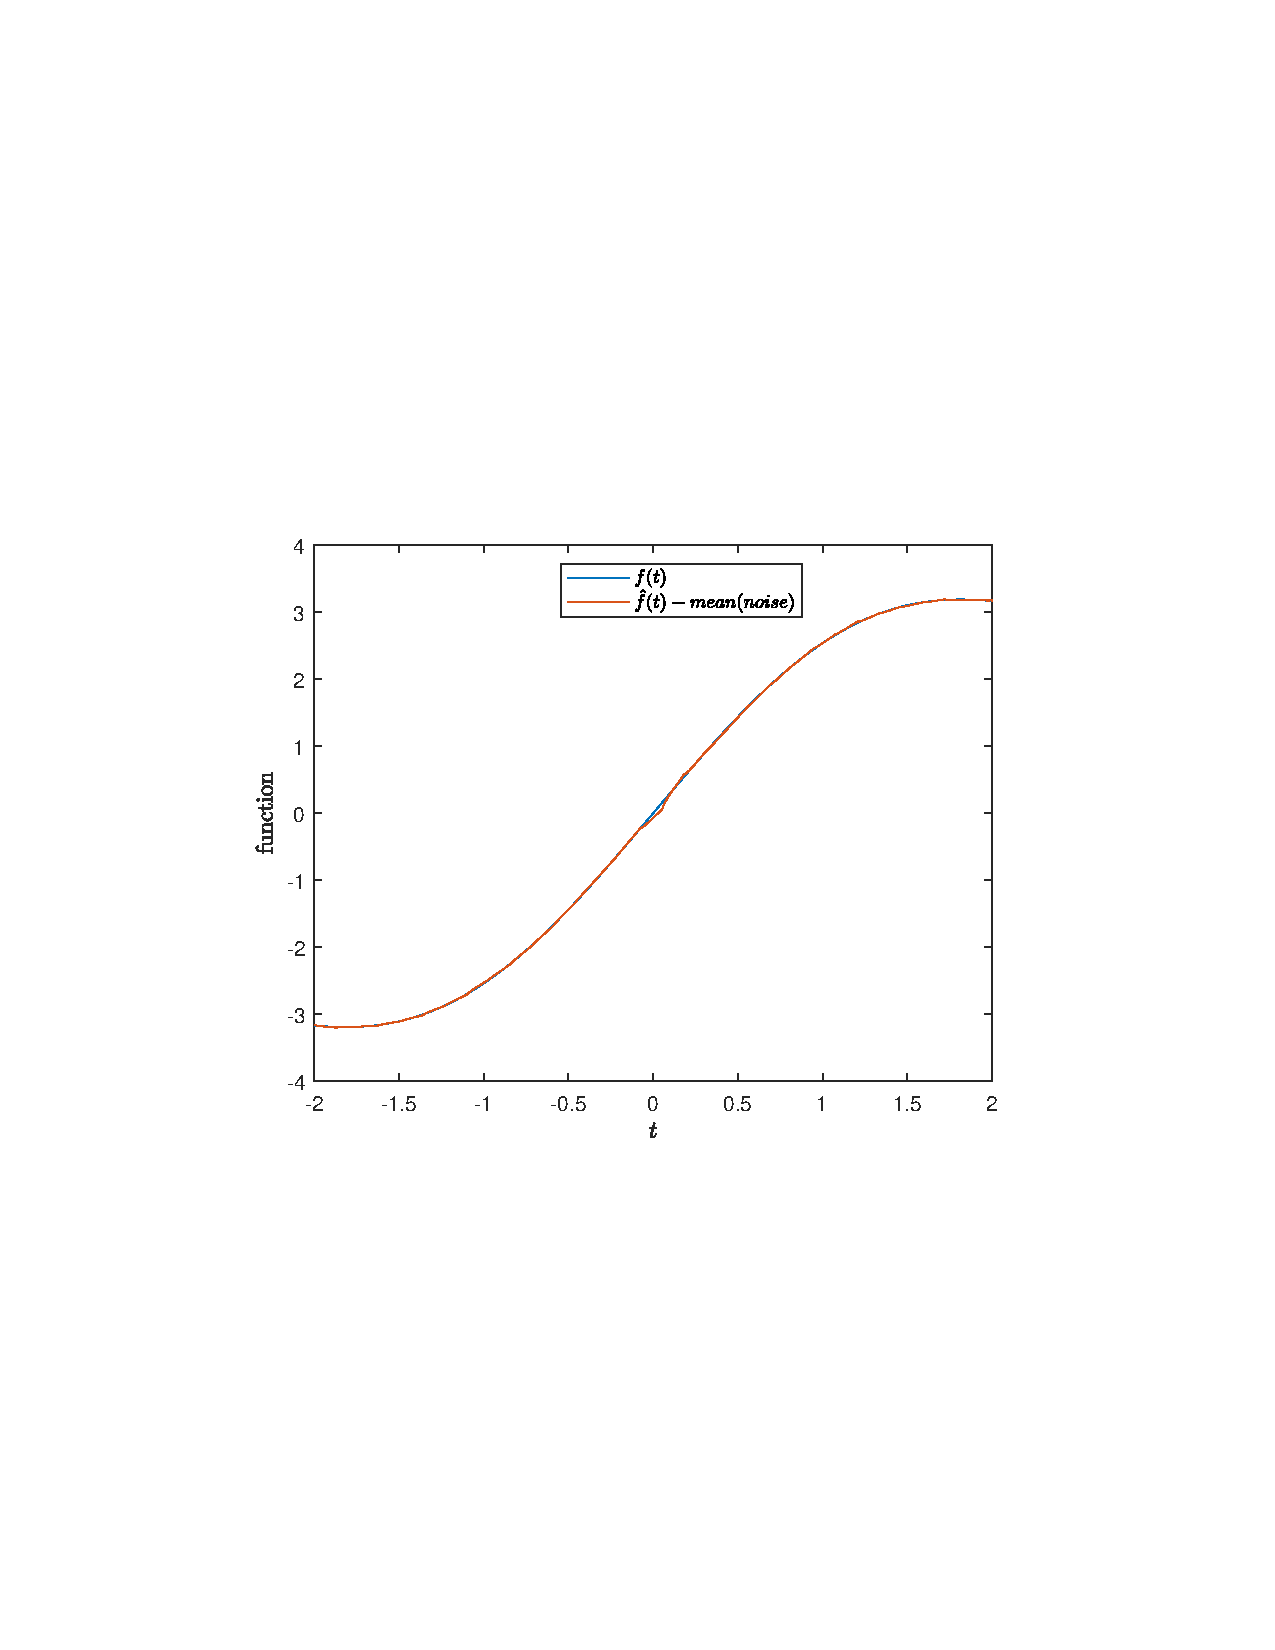
\includegraphics[trim={3.5cm 8cm 4cm 9cm},clip,width=1\textwidth]{Images/HardFunc.pdf}
	\caption{Plot of clean and reconstructed signal. $\delta = 0.501$. For Hard thresholding}
	\label{sub:BestDeltaFunc}
\end{subfigure}
\begin{subfigure}{0.49\textwidth}
	\centering
	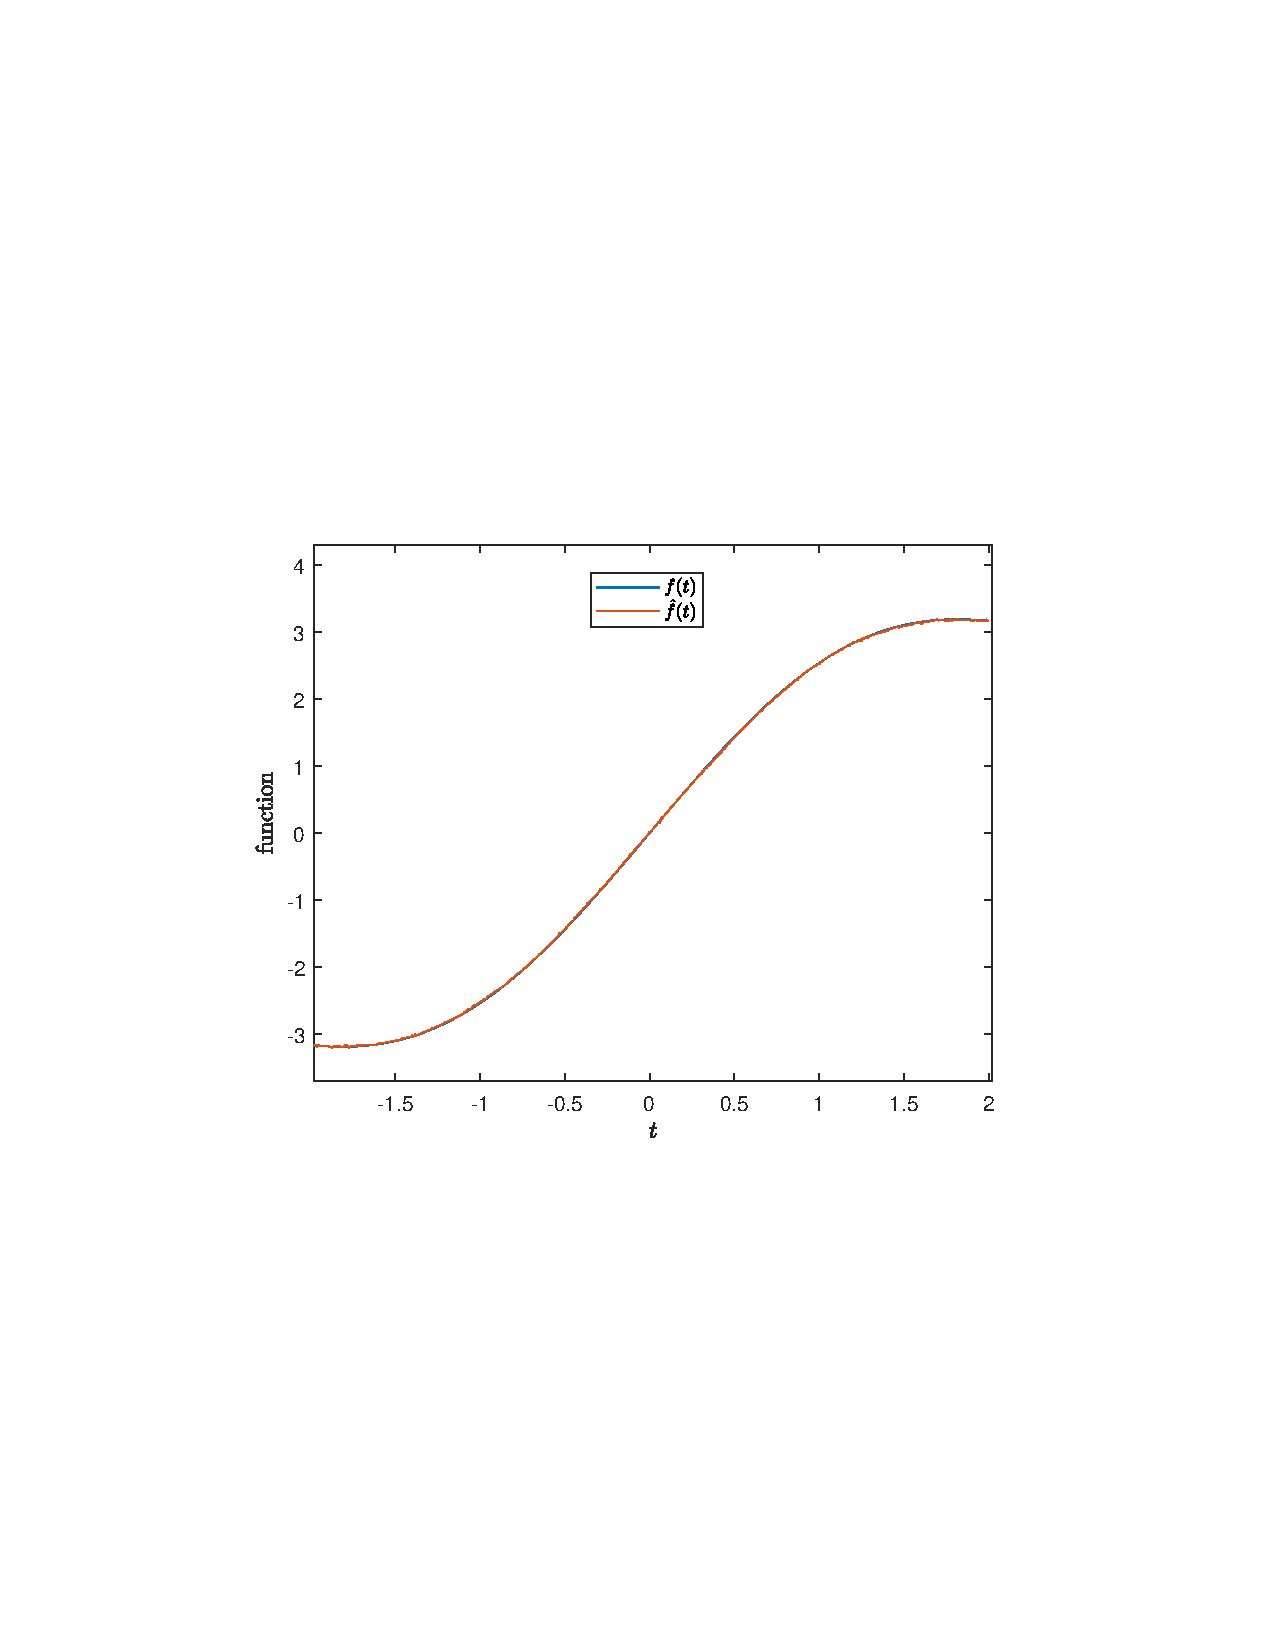
\includegraphics[trim={3.5cm 8cm 4cm 9cm},clip,width=1\textwidth]{Images/SoftFunc.pdf}
	\caption{Plot of clean and reconstructed signal. $\delta = 0.0398$. For soft threasholding}
	\label{sub:BestDeltaSoftFunc}
\end{subfigure}
\caption{Plots for the recontructed functions, via different type of thresholding}
\label{fig:OptiDelta}
\end{figure}

    \subsection{Images with noise}

    \subsubsection{Task 2.4} \label{subsubsec:Denoising}
	An image is composed of 3 different matrices, each representing the value of the color red,blue and green. To denoise an image, the following steps will be executed:
	\begin{enumerate}
		\item Separate image (multidimensional array) into 3 matrices representing the 3 RGB colors
		\item Compute the 2D wavelet transform using matlab \texttt{wavedec2} for each of the 3 matrices. We will then have 3 different wavelet coefficient array's.
		\item Apply a thresholding scheme to the wavelet coefficients, for the 3 different colors (arrays)
		\item Compute the inverse 2D wavelet transform using matlab \texttt{wavrec2}, for the 3 different colors (arrays)
		\item Recombine the denoised color matrices into 1 image (multidimensional array)
	\end{enumerate}
	Since we are dealing with image denoising, the wavelet families to test on are Daubechies or biorthogonal CDF's. \\

	We will test the wavelet-based denoising scheme on a picture (\cref{sub:Bib}) for different thresholds (using hard thesholding), BiorSplines4.4 as wavelet and decomposition level of 4. The resulting figures are in \cref{fig:Bib}, \cref{tab:bib} summarizes the results. We can clearly see as the threshold is increased, the error (Frobenius) and compression ration increase as well. This is expected as a higher threshold results in more of the (signal) picture being thrown away.

\begin{table}[H]
	\centering
	\begin{tabular}{|l|l|l|l|}
	\hline
	$\delta$	& Compression ratio & $\|A-\tilde{A}\|_F$ & $\frac{\|A-\hat{A}\|_F}{\|A\|_F}$ \\ \hline
	4.32	& 1.95 & \texttt{2.37e+03} & \texttt{0.0097} \\ \hline
	43.205	& 9.73 & \texttt{2.38e+04} & \texttt{0.097} \\ \hline
	432.048	& 219.84 & \texttt{6.805e+04} & \texttt{0.28} \\ \hline
	\end{tabular}
	\caption{Table summarizing the results for different threshold values, tested on \cref{sub:Bib}. Using BiorSplines4.4 as wavelet and decomposition level of 4. $\hat{A}$ is the reconstructed image}
	\label{tab:bib}
\end{table}

\begin{figure}[H]
	\centering
	\begin{subfigure}{0.49\textwidth}
		\centering
		%trim={<left> <lower> <right> <upper>}
		%\includegraphics[trim={4cm 8cm 4cm 8cm},clip,width=.49\textwidth]{Images/LQG_weighted4.pdf}
		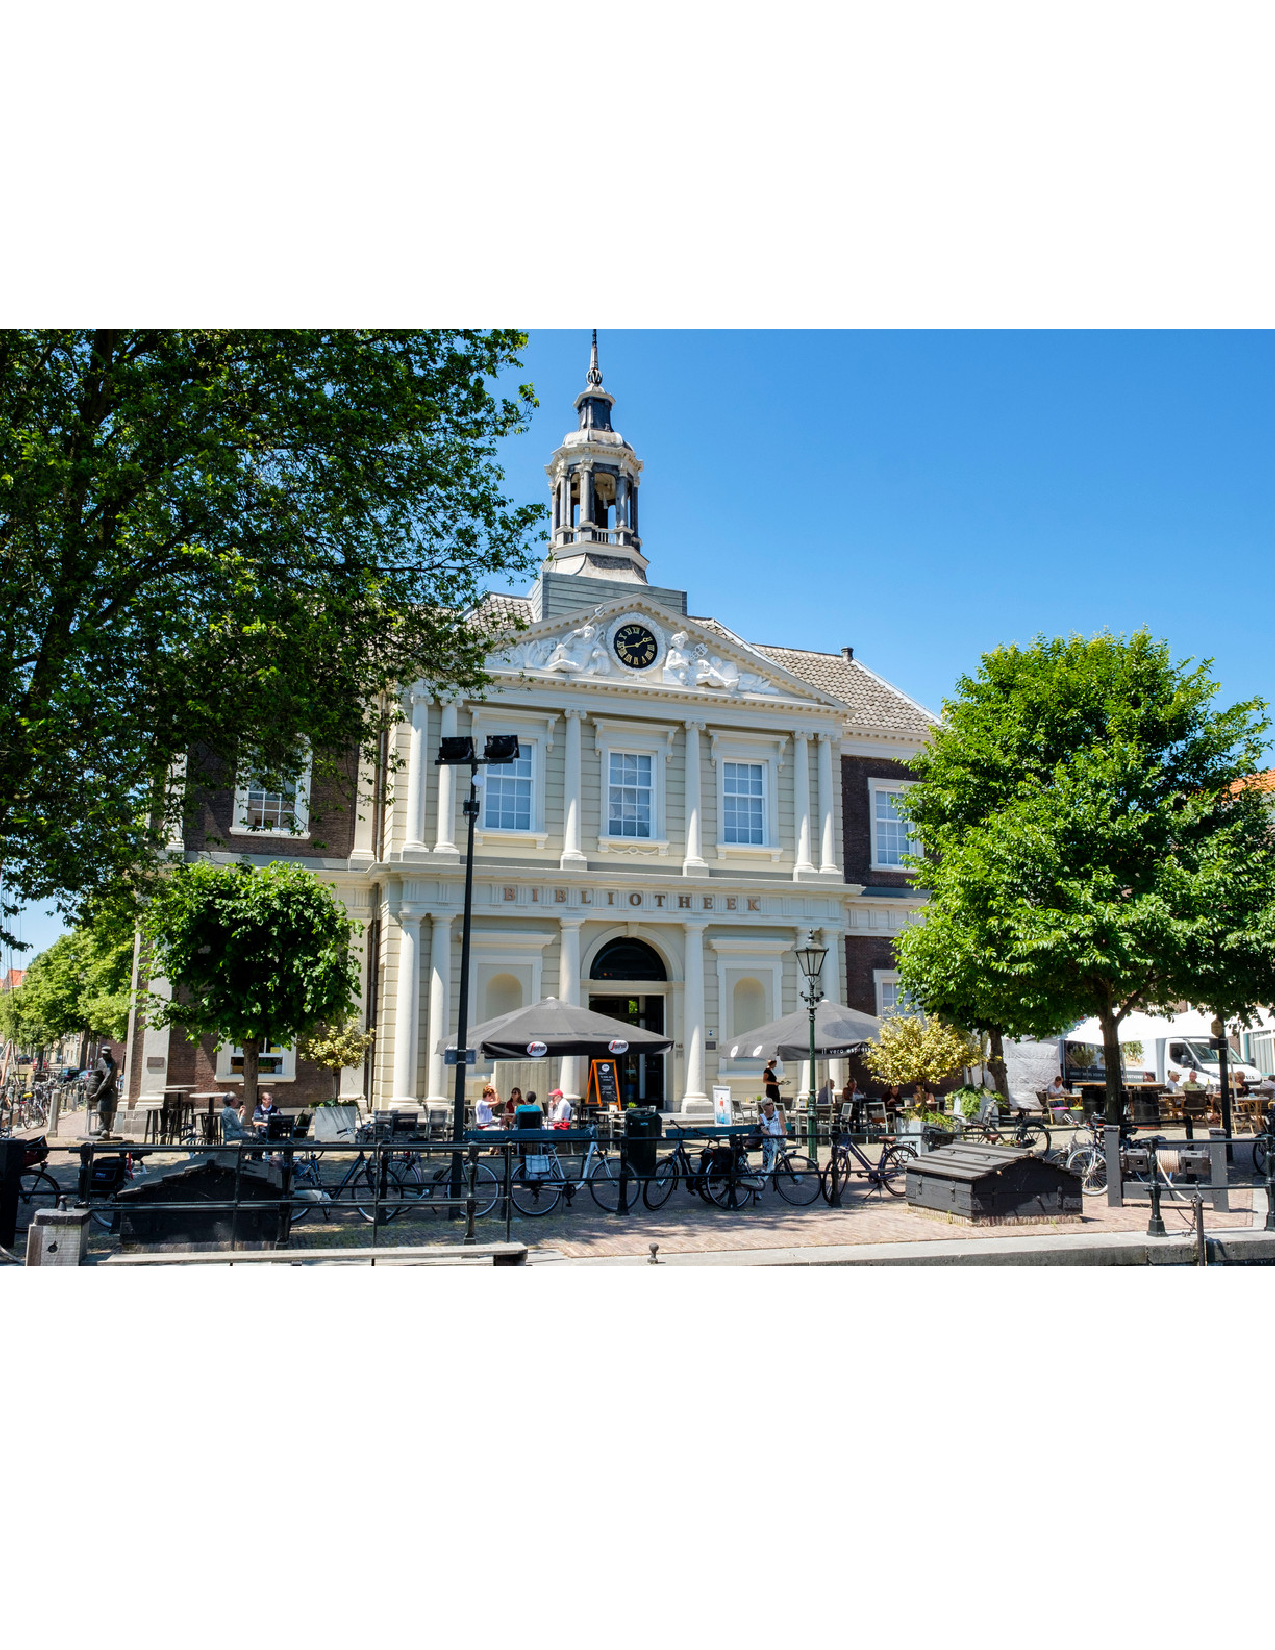
\includegraphics[trim={4cm 8cm 4cm 8cm},clip,width=1\textwidth]{Images/Bib.pdf}
		\caption{Picture of a library, original}
		\label{sub:Bib}
	\end{subfigure}
	\begin{subfigure}{0.49\textwidth}
	\centering
	%trim={<left> <lower> <right> <upper>}
	%\includegraphics[trim={4cm 8cm 4cm 8cm},clip,width=.49\textwidth]{Images/LQG_weighted4.pdf}
	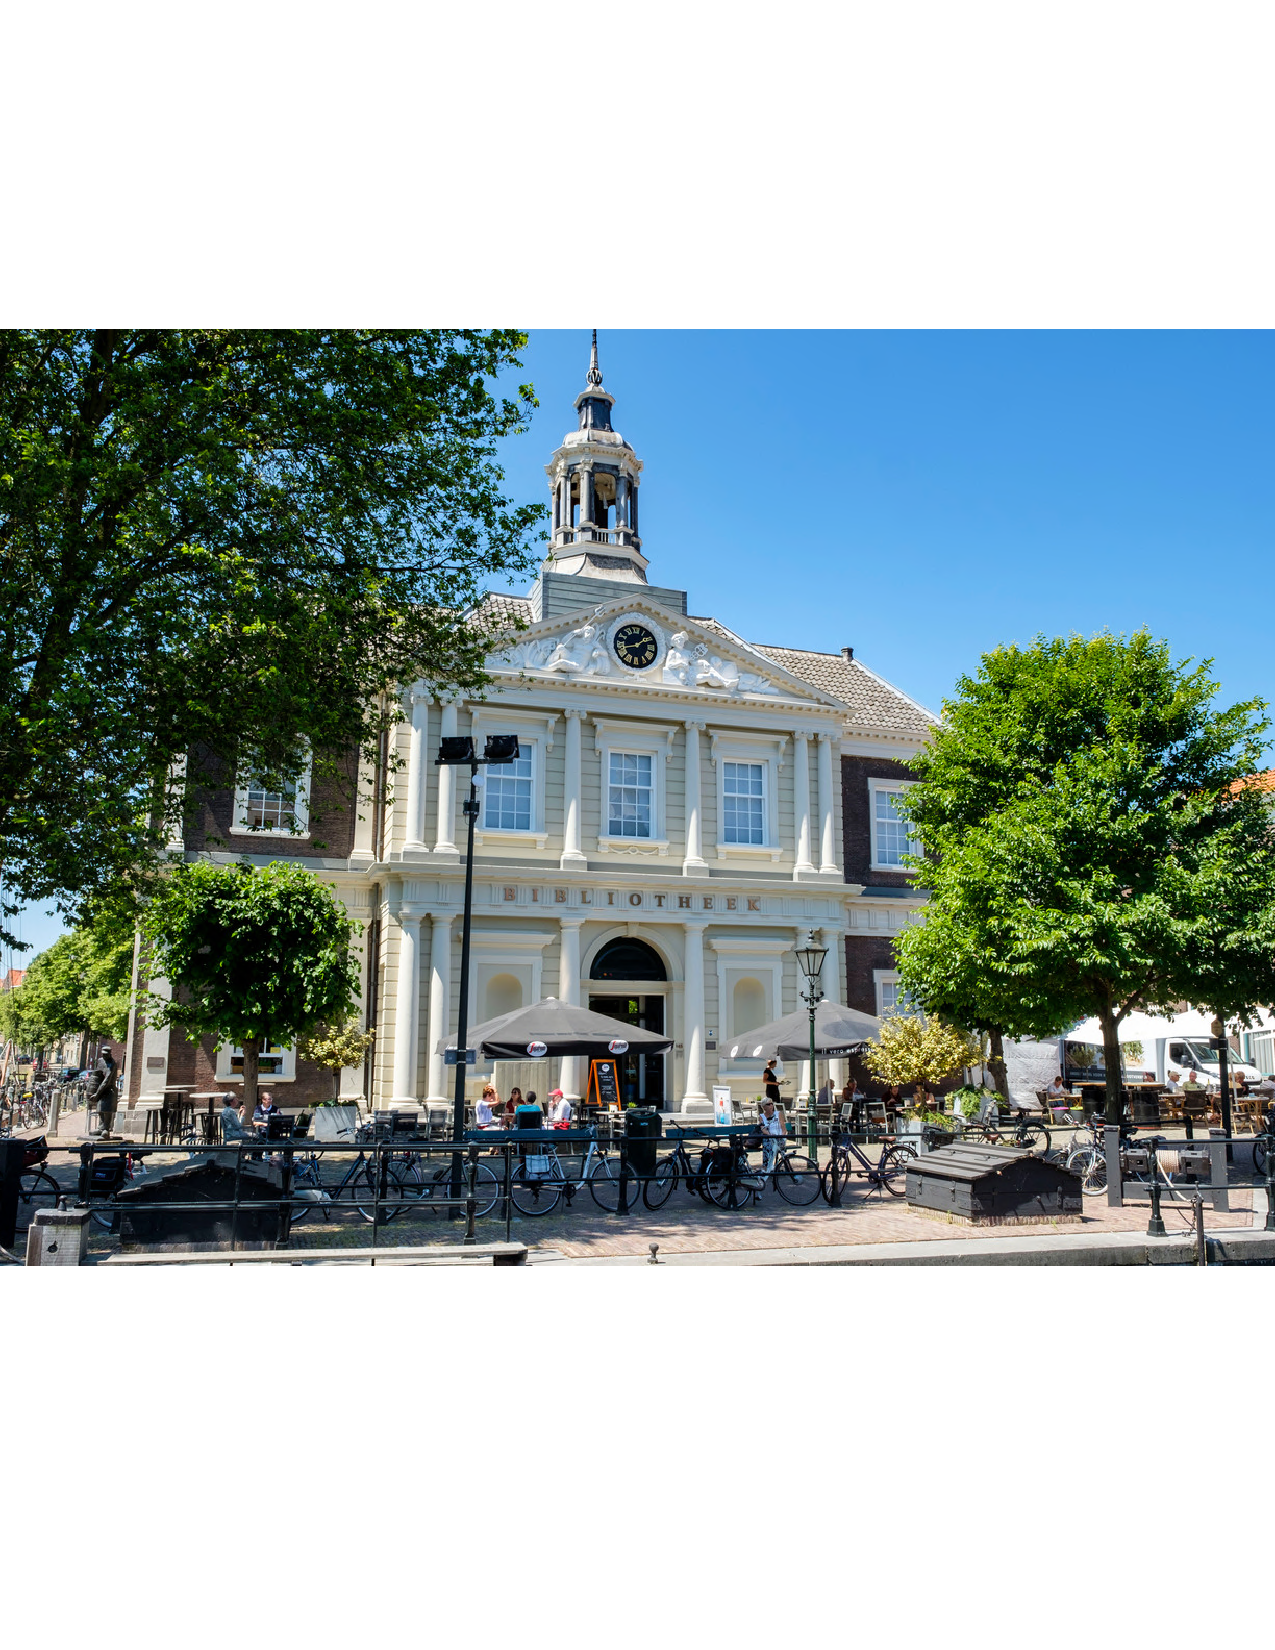
\includegraphics[trim={4cm 8cm 4cm 8cm},clip,width=1\textwidth]{Images/BibGood.pdf}
	\caption{Picture of a library, $\delta = 4.32$}
	\label{sub:BibGood}
\end{subfigure}
	\begin{subfigure}{0.49\textwidth}
	\centering
	%trim={<left> <lower> <right> <upper>}
	%\includegraphics[trim={4cm 8cm 4cm 8cm},clip,width=.49\textwidth]{Images/LQG_weighted4.pdf}
	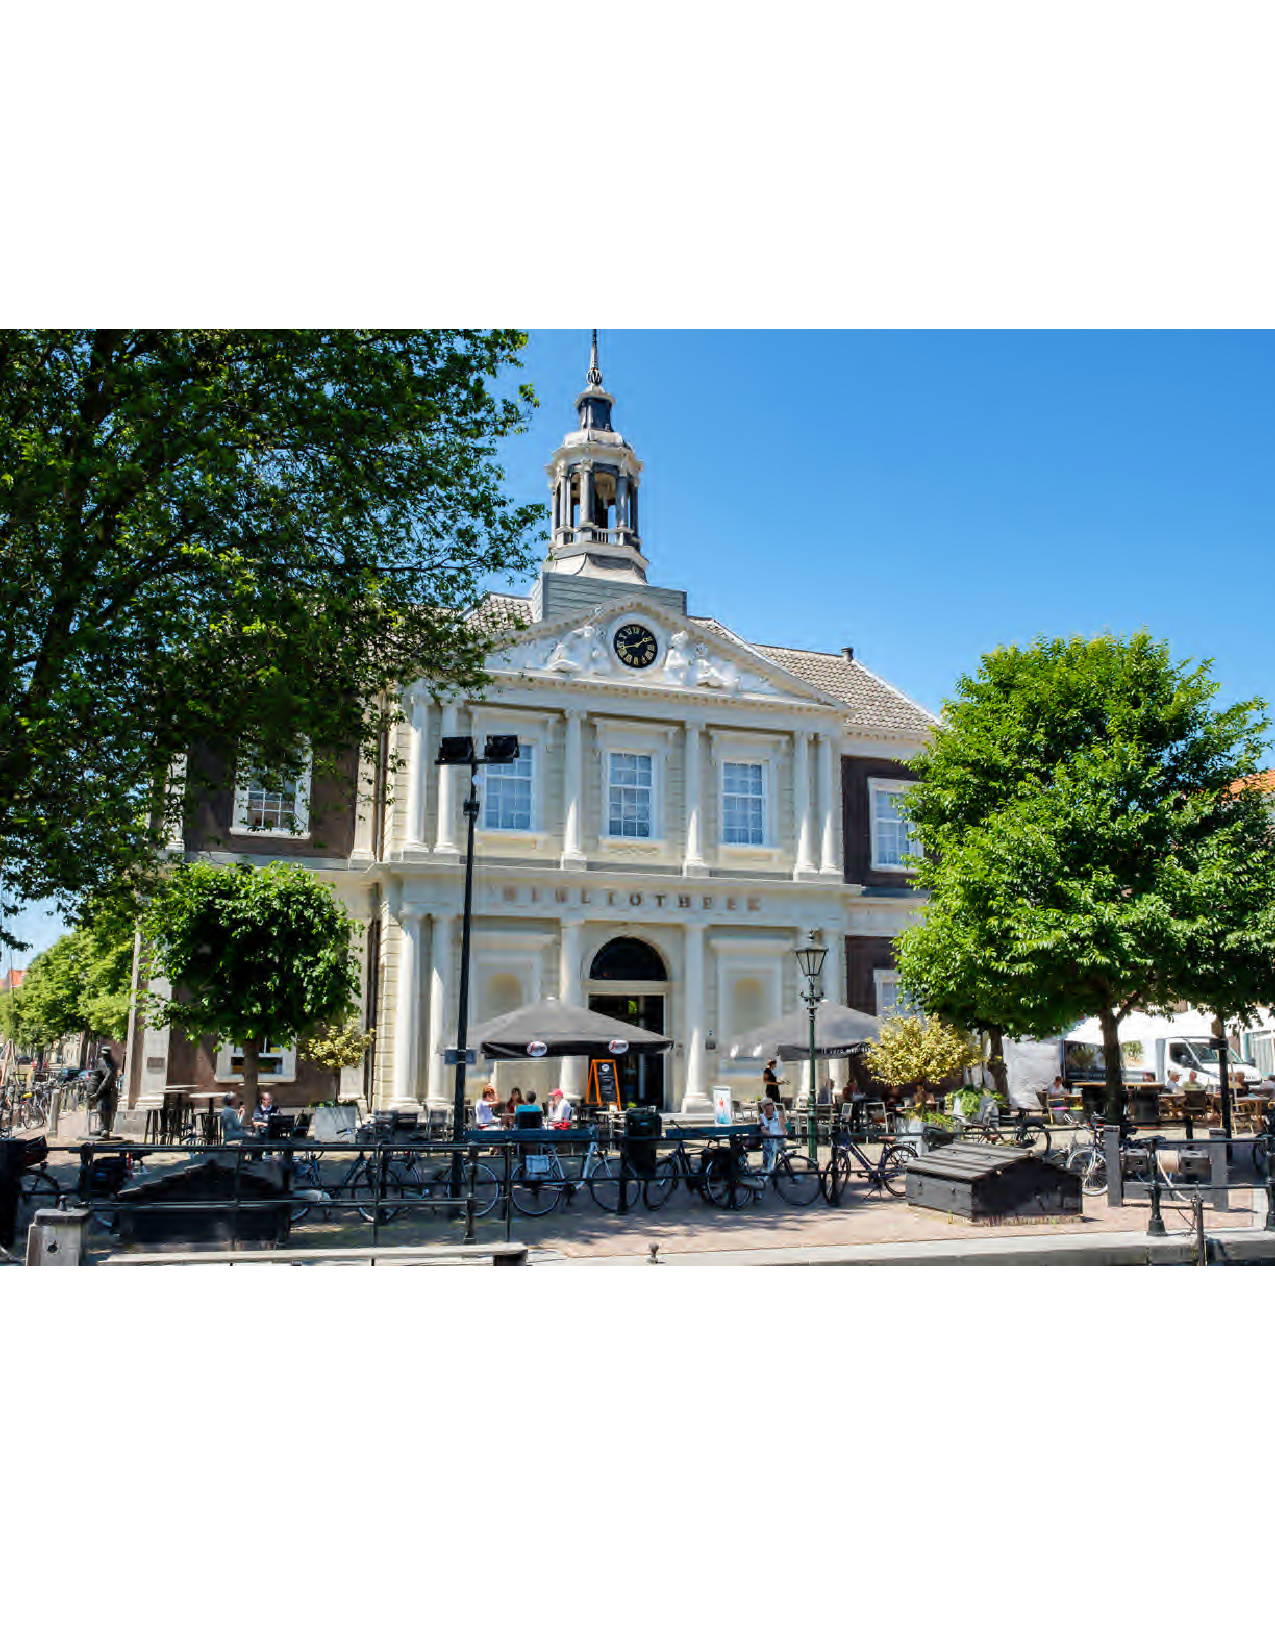
\includegraphics[trim={4cm 8cm 4cm 8cm},clip,width=1\textwidth]{Images/BibMid.pdf}
	\caption{Picture of a library, $\delta = 43.205$}
	\label{sub:BibMid}
\end{subfigure}
	\begin{subfigure}{0.49\textwidth}
	\centering
	%trim={<left> <lower> <right> <upper>}
	%\includegraphics[trim={4cm 8cm 4cm 8cm},clip,width=.49\textwidth]{Images/LQG_weighted4.pdf}
	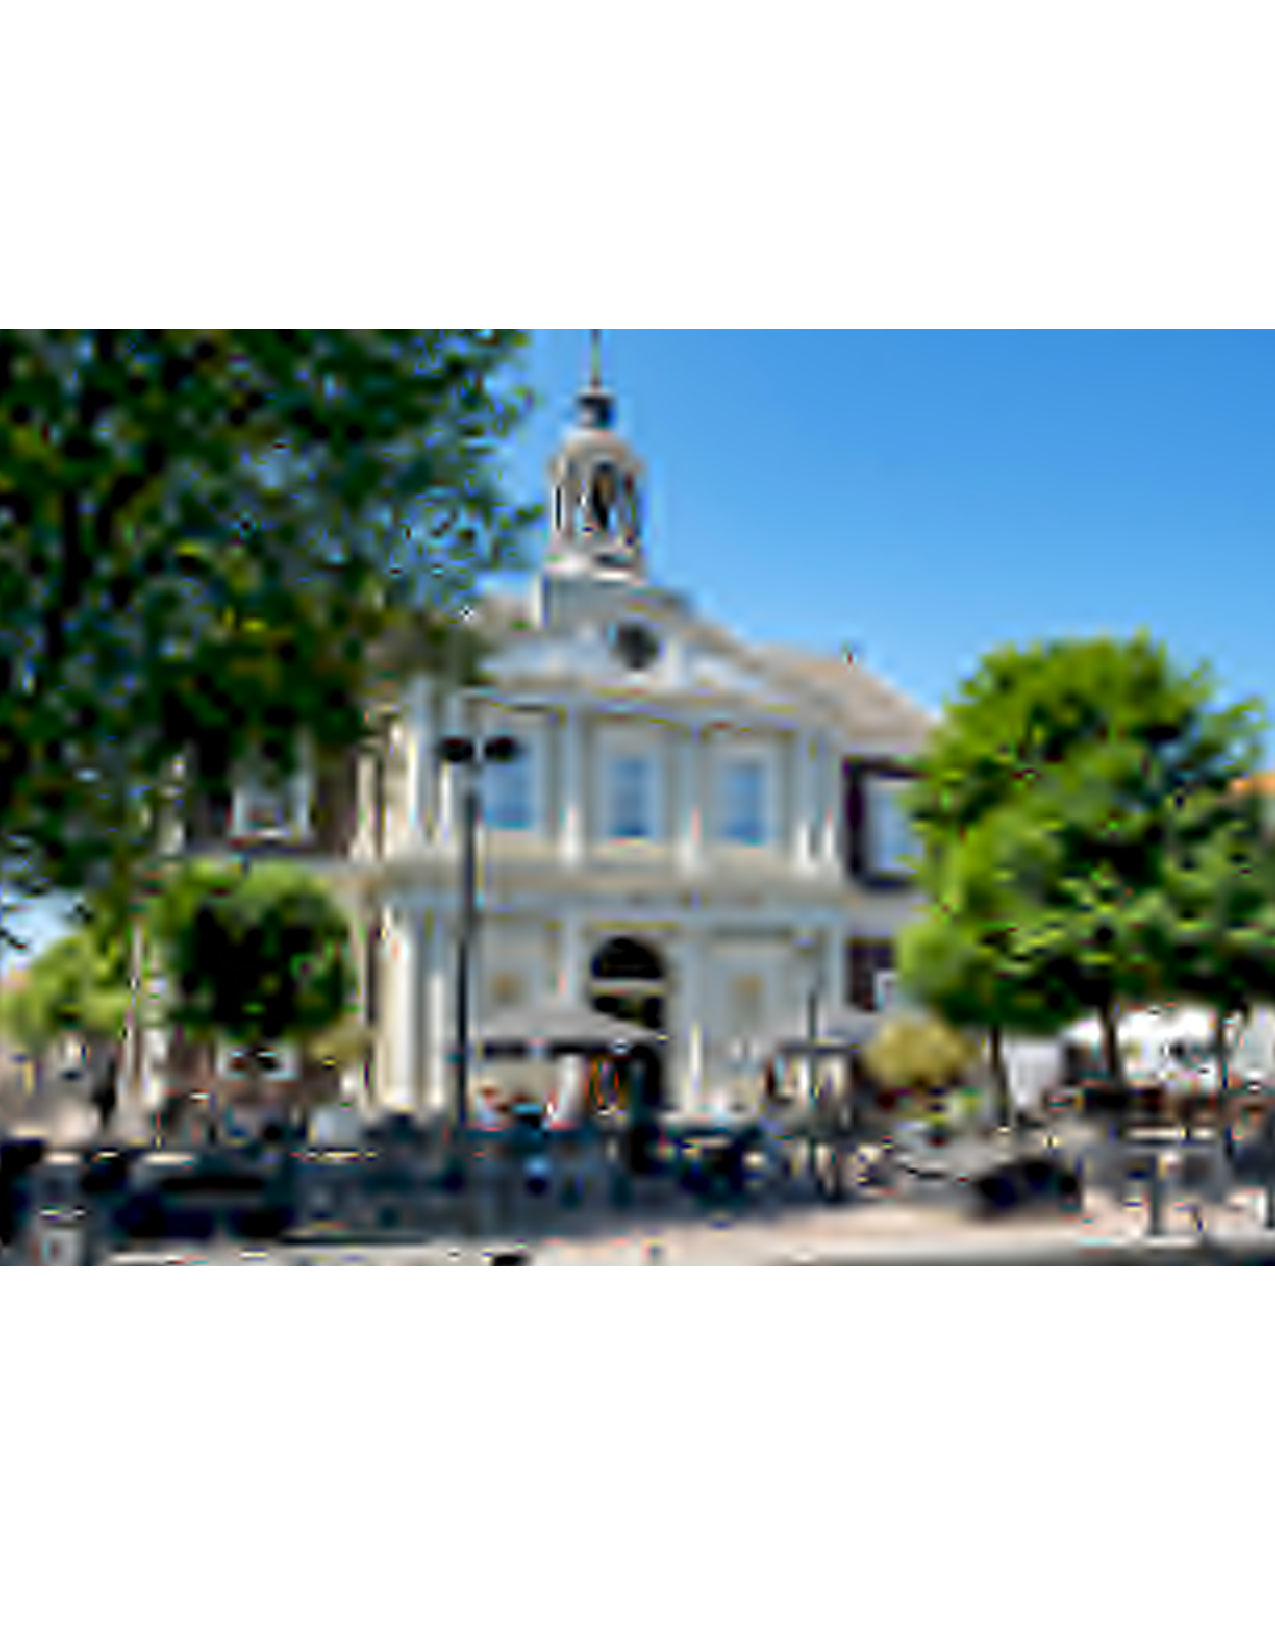
\includegraphics[trim={4cm 8cm 4cm 8cm},clip,width=1\textwidth]{Images/BibBad.pdf}
	\caption{Picture of a library, $\delta = 432.048$}
	\label{sub:BibBad}
\end{subfigure}
	\caption{Picture of a library (taken from personal phone), for different values of hard threshold. Using BiorSplines4.4 as wavelet and decomposition level of 4}
	\label{fig:Bib}
\end{figure}

    \subsubsection{Question 2.5} \label{subsubsec:stdWave}

	We will now add salt and pepper noise to \cref{sub:Bib} via matlab \texttt{imnoise(I,'salt \& pepper',0,01)} function, with 0.01 as noise density (affects approximately 0.01 times the number of pixels). The noisy image looks like \cref{fig:Noisy}, it has an SNR (signal to noise ratio) of 9.301 and clearly looks noisy. The SNR was computed via
	\begin{equation} \label{eq:SNR}
		\texttt{SNR} = 10 \log_{10}{\frac{\|A\|_F}{\|A-\hat{A}\|_F}}
	\end{equation}
	With $A$ the multidimensional array representing the image, $\hat{A}$ the reconstructed or noisy image.
    \begin{figure}[H]
	\centering
	\includegraphics[trim={0cm 6cm 0cm 5.5cm},clip,width=0.7\textwidth]{Images/NoisyBib.pdf}
	\caption{\cref{sub:Bib} with salt and pepper noise fo density 0.01, added via matlab \texttt{imnoise(I,'salt \& pepper',0,01)}}
	\label{fig:Noisy}
\end{figure}

	We will test the denosing procedure for both hard and soft thresholding, for a range of $\delta = p T$'s, with $T$ the max of the wavelet coefficients of the 3 RGB colors and $p \in [0,1]$. 10 equidistant $p$'s were tested, obtained from matlab \texttt{linspace(\texttt{1e-3},1,10)}. \\
	The tested wavelets range from (For 4 level deep)
	\begin{itemize}
		\item Daubechies (orthogonal): \texttt{"db1",...,"db45"}
		\item BiorSplines (biorthgonal): \texttt{"bior1.1", "bior1.3", "bior1.5"
			"bior2.2", "bior2.4", "bior2.6", "bior2.8"
			"bior3.1", "bior3.3", "bior3.5", "bior3.7"
			"bior3.9", "bior4.4", "bior5.5", "bior6.8"}	
		\item ReverseBior (biorthogonal): \texttt{	"rbio1.1", "rbio1.3", "rbio1.5"
			"rbio2.2", "rbio2.4", "rbio2.6", "rbio2.8"	
			"rbio3.1", "rbio3.3", "rbio3.5", "rbio3.7"
			"rbio3.9", "rbio4.4", "rbio5.5", "rbio6.8"}
	\end{itemize}
	1500 different combinations were tested, only the best will be shown (for obvious reasons) \footnote{To run the tests and recreate \cref{fig:Bib,fig:Noisy,fig:RecBib,fig:CusBib}, run \texttt{ex2point2.m}} \\
	
	The best parameters will be determined using the SNR metric (the higher the better), of course in practice the clean image is usually not available, so the "eyeball" norm would have to be use. The best parameters according to \texttt{SNR} are: \texttt{db45} for the wavelet, threshold of 4.902 and a $\texttt{SNR} = \texttt{9.8}$, using soft thresholding. See \cref{fig:RecBib} for the resulting recontructed image. It still looks quite noisy figure. The results are pretty underwhelming.

    \begin{figure}[H]
	\centering
	\includegraphics[trim={0cm 6cm 0cm 5.5cm},clip,width=0.7\textwidth]{Images/RecontructedBib.pdf}
	\caption{Recontructed image from \cref{fig:Noisy}. Using threshold of 4.902, hard thresholding and \texttt{db45} for the wavelet}
	\label{fig:RecBib}
\end{figure}
	
	Let us take a trial and error approach with the eyeball norm as quality metric. we get the following parameters: threshold of 28.15, \texttt{db30} as wavelet and \texttt{SNR = 8.89} using soft thresholding. As we can see in \cref{fig:CusBib}, the image feels less noisy but more blurry.
	
    \begin{figure}[H]
	\centering
	\includegraphics[trim={0cm 6cm 0cm 5.5cm},clip,width=0.7\textwidth]{Images/CustomBib.pdf}
	\caption{Recontructed image from \cref{fig:Noisy}. Using threshold of 41.71, soft thresholding and \texttt{db30} for the wavelet}
	\label{fig:CusBib}
\end{figure}
	
	The better image is a matter of preference, noisy vs blurry, whichever one is preferred. If just the \texttt{SNR} metric is used, then \cref{fig:RecBib}, is optimal.
	
	\begin{comment}
\begin{table}[H]
	\centering
	\begin{tabular}{|l|l|l|l|l|l|l|l|l|l|l|}
		\hline
		$p$	& 0.001 &   0.11 &   0.22  &  0.33 &   0.44 &   0.56  &  0.68 &   0.78  &  0.89   & 1 \\ \hline
		\texttt{db1} & & & & & & & & & & \\ \hline
	\end{tabular}
	\caption{Table summarizing the SNR results for different threshold values, tested on \cref{sub:Bib}. Using BiorSplines4.4 as wavelet and decomposition level of 4}
	\label{tab:ImageNoise}
\end{table}
	\end{comment}
	
	%However the parameters are not generalizable since these are the best parameters for this denoising this specific image with gaussian noise, for different type of noise and image the optimal parameters might be different.
	
    \subsection{Using a redundant wavelet transform}

    \subsubsection{Task 2.6}

	An image is composed of 3 different matrices, each representing the value of the color red,blue and green. To denoise an image, the following steps will be executed:
\begin{enumerate}
	\item Separate image (multidimensional array) into 3 matrices representing the 3 RGB colors
	\item Compute the 2D stationary wavelet transform using matlab \texttt{swt2} for each of the 3 matrices. The ouptut of the \texttt{swt2} gives us a multidimensional array, containing the approximation and detail coefficients
	\item Apply a thresholding scheme to the approximation and detail coefficients, for the 3 different colors (multidimensional arrays)
	\item Compute the inverse 2D stationary wavelet transform matlab \texttt{iswt}, for the 3 different colors (multidimensional arrays)
	\item Recombine the denoised color matrices into 1 image (multidimensional array)
\end{enumerate}

    \subsubsection{Question 2.7}
	Since we are dealing with image denoising, the wavelet families to test on are Daubechies or biorthogonal CDF's. \\

	We will test the redundant wavelet-based denoising scheme on \cref{fig:Noisy}, for both hard and soft thresholding, for a range of $\delta = p T$'s, with $T$ the max of the wavelet coefficients of the 3 RGB colors and $p \in [0,1]$. 10 equidistant $p$'s were tested, obtained from matlab \texttt{linspace(\texttt{1e-3},1,10)}. \\
The tested wavelets range from (For 4 level deep)
\begin{itemize}
	\item Daubechies (orthogonal): \texttt{"db1",...,"db45"}
	\item BiorSplines (biorthgonal): \texttt{"bior1.1", "bior1.3", "bior1.5"
		"bior2.2", "bior2.4", "bior2.6", "bior2.8"
		"bior3.1", "bior3.3", "bior3.5", "bior3.7"
		"bior3.9", "bior4.4", "bior5.5", "bior6.8"}	
	\item ReverseBior (biorthogonal): \texttt{	"rbio1.1", "rbio1.3", "rbio1.5"
		"rbio2.2", "rbio2.4", "rbio2.6", "rbio2.8"	
		"rbio3.1", "rbio3.3", "rbio3.5", "rbio3.7"
		"rbio3.9", "rbio4.4", "rbio5.5", "rbio6.8"}
\end{itemize}
1500 different combinations were tested, only the best for the redundant scheme will be shown (for obvious reasons) \footnote{To run the tests and recreate \cref{fig:RecRed,fig:RecCus}, run \texttt{ex2point3.m}}. The quality metric is \texttt{SNR} (The higher the better), see \cref{eq:SNR}.\\

%The best parameters for standard wavelet transform are: threshold of 42, using hard thesholding, wavelet is \texttt{"db1"} .We get \texttt{SNR = }, see \cref{sub:RecStd}.\\
The best parameters for redundant wavelet transform are: threshold of 1.508, using soft thesholding, wavelet is \texttt{"db45"}.We get \texttt{SNR = 9.49}, see \cref{fig:RecRed}. The resulting figure still has quite a bit of noise. 	Compared to the standard wavelet transform in \cref{subsubsec:stdWave}, the redundant is slightly worse for similar parameters w/r to \texttt{SNR} metric.\\

    \begin{figure}[H]
	\centering
	\includegraphics[trim={0cm 6cm 0cm 5.5cm},clip,width=0.7\textwidth]{Images/BibRecRed.pdf}
	\caption{Recontructed image from \cref{fig:Noisy}. Using redundant wavelet transform, a threshold of 1.508, soft thresholding and \texttt{db45} for the wavelet}
	\label{fig:RecRed}
\end{figure}

	Let us take a trial and error approach with the eyeball norm as quality metric. we get the following parameters: threshold of 26.73, \texttt{db30} as wavelet and \texttt{SNR = 9.204} using soft thresholding. As we can see in \cref{fig:RecCus}, the image is less noisy but more blurry. Compared to the standard wavelet transform in \cref{subsubsec:stdWave}, the redundant is slightly better for similar parameters w/r to \texttt{SNR} metric.

    \begin{figure}[H]
	\centering
	\includegraphics[trim={0cm 6cm 0cm 5.5cm},clip,width=0.7\textwidth]{Images/BibRecCus.pdf}
	\caption{Recontructed image from \cref{fig:Noisy}. Using redundant wavelet transform, a threshold of 26.73, soft thresholding and \texttt{db30} for the wavelet}
	\label{fig:RecCus}
\end{figure}

	 When comparing \cref{fig:RecCus,fig:RecRed}, even though \cref{fig:RecRed} has the higher \texttt{SNR}, \cref{fig:RecCus} looks like it has less noise. This is due to the fact that the additional blur and lowering in quality is too much of a price to pay to denoise properly, according to \texttt{SNR}.

    \subsubsection{Question 2.8}

	Let us take \cref{eq:func} again, this time however for $N=1008$ points in the interval $[-2,2]$ (obtained via matlab \texttt{linspace(-2,2,1008)}). Noise is added to the signal 
	\begin{equation} \label{eq:funcNoise}
		\tilde{f_i} = f_i + \epsilon \mathcal{N}(0,1)
	\end{equation}
	($\hat{f}$ is the reconstructed $\tilde{f}$). We chose $\epsilon = \texttt{5e-1}$. See \footnote{To recreate \cref{fig:FuncNoisy,fig:FuncRecStd,fig:FuncRecRed}, run \texttt{ex2point31.m}} \cref{fig:FuncNoisy} for signal plot.\\
	
	On this slightly modified signal both redundant and standard wavelet transform will be tested, for wavelet \texttt{db2}, Level of decomposition 4, both hard and soft thresholding and a range of $\delta = p T$'s, with $T$ the max of the wavelet coefficients and $p \in [0,1]$. 400 equidistant $p$'s were tested, obtained from matlab \texttt{linspace(0,1,400)}. Boundary conditions used is still: Symmetrization (half-point). \\
	
	The measure of quality will be \text{SNR} \cref{eq:SNR} (the higher the better), with $\hat{f}$ and $f$ replacing $\hat{A}$ and $A$ respectively. The \texttt{SNR} of the noise is 6.65.

    \begin{figure}[H]
	\centering
	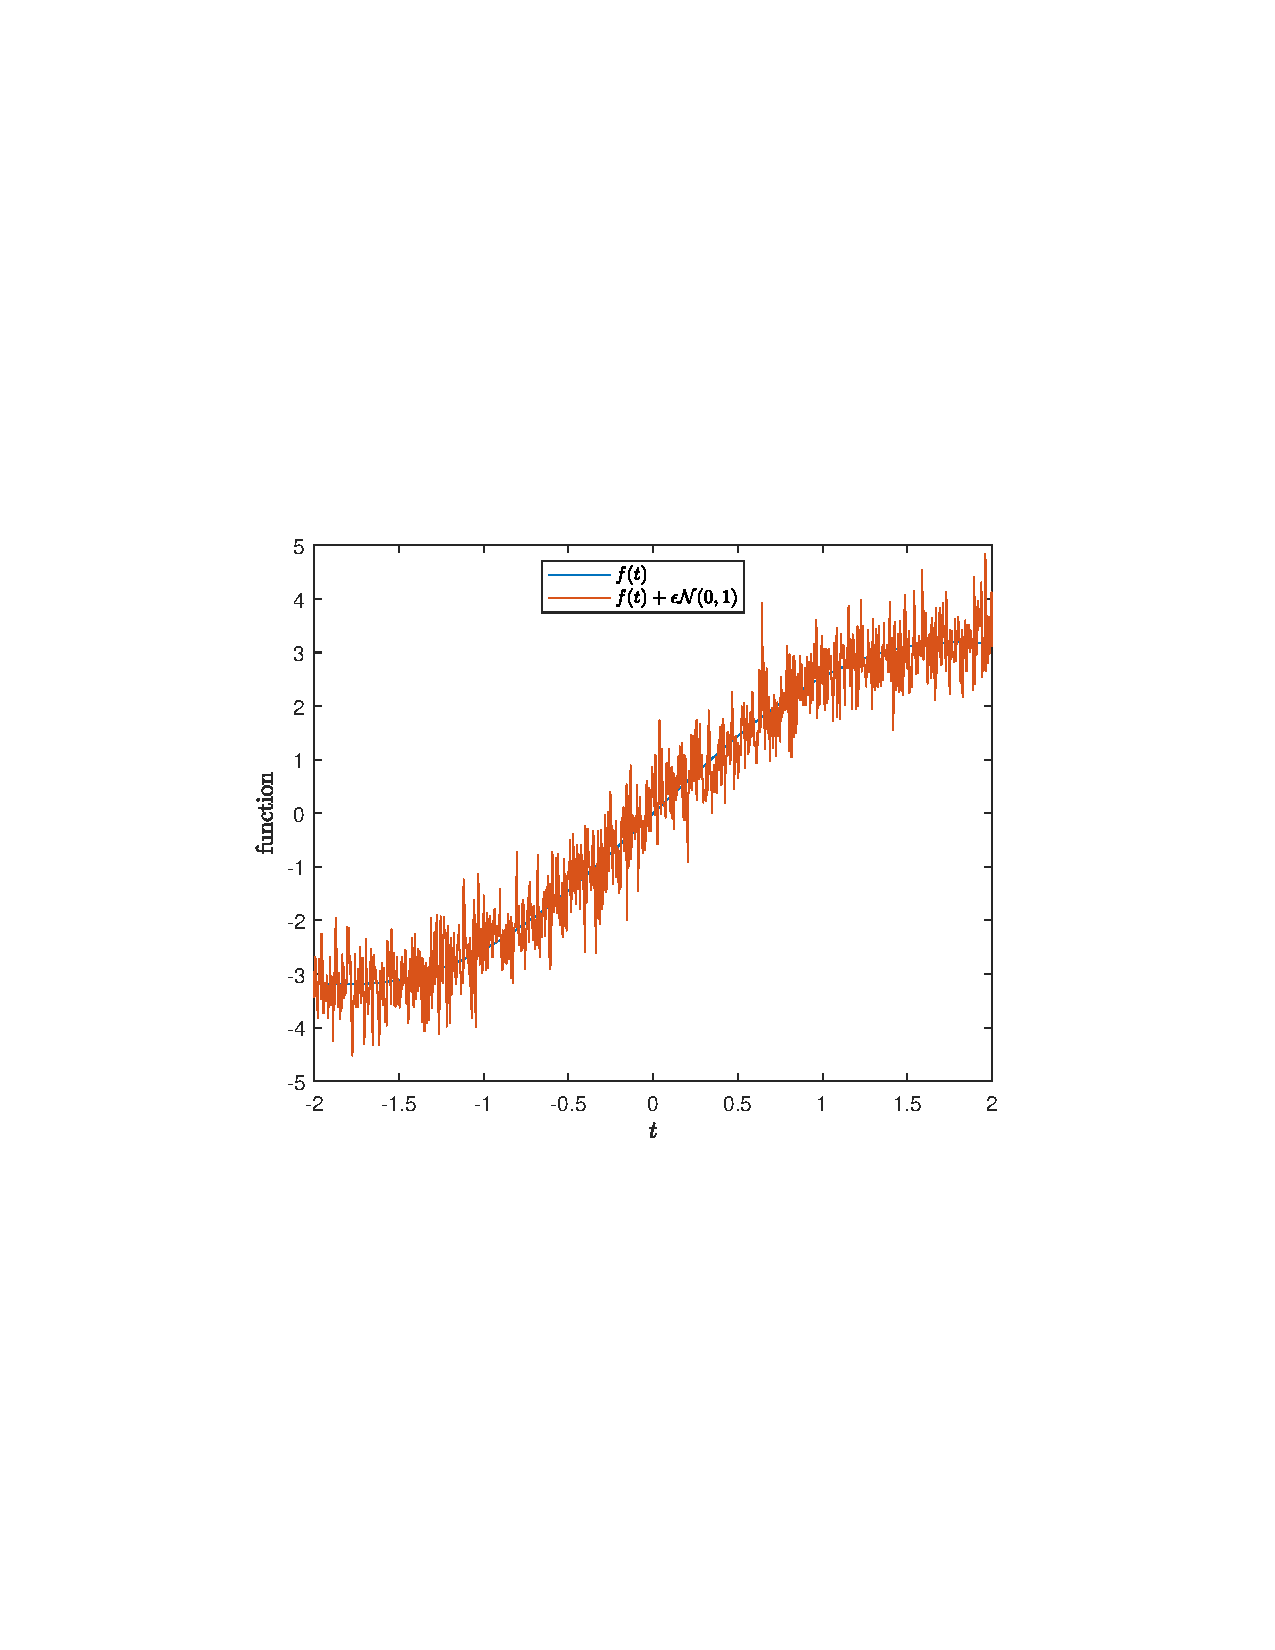
\includegraphics[trim={3.5cm 8cm 4cm 9cm},clip,width=0.7\textwidth]{Images/FuncNoisy.pdf}
	\caption{Plot of function \cref{eq:func}, and it's noisy counterpart \cref{eq:funcNoise}}
	\label{fig:FuncNoisy}
	\end{figure}

	The best threshold for the standard wavelet transform is 1.73, using hard thresholding. \texttt{SNR=12.55}. See \cref{fig:FuncRecStd} for results.
\begin{figure}[H]
	\centering
	\begin{subfigure}{0.49\textwidth}
		\centering
		%trim={<left> <lower> <right> <upper>}
		%\includegraphics[trim={4cm 8cm 4cm 8cm},clip,width=.49\textwidth]{Images/LQG_weighted4.pdf}
		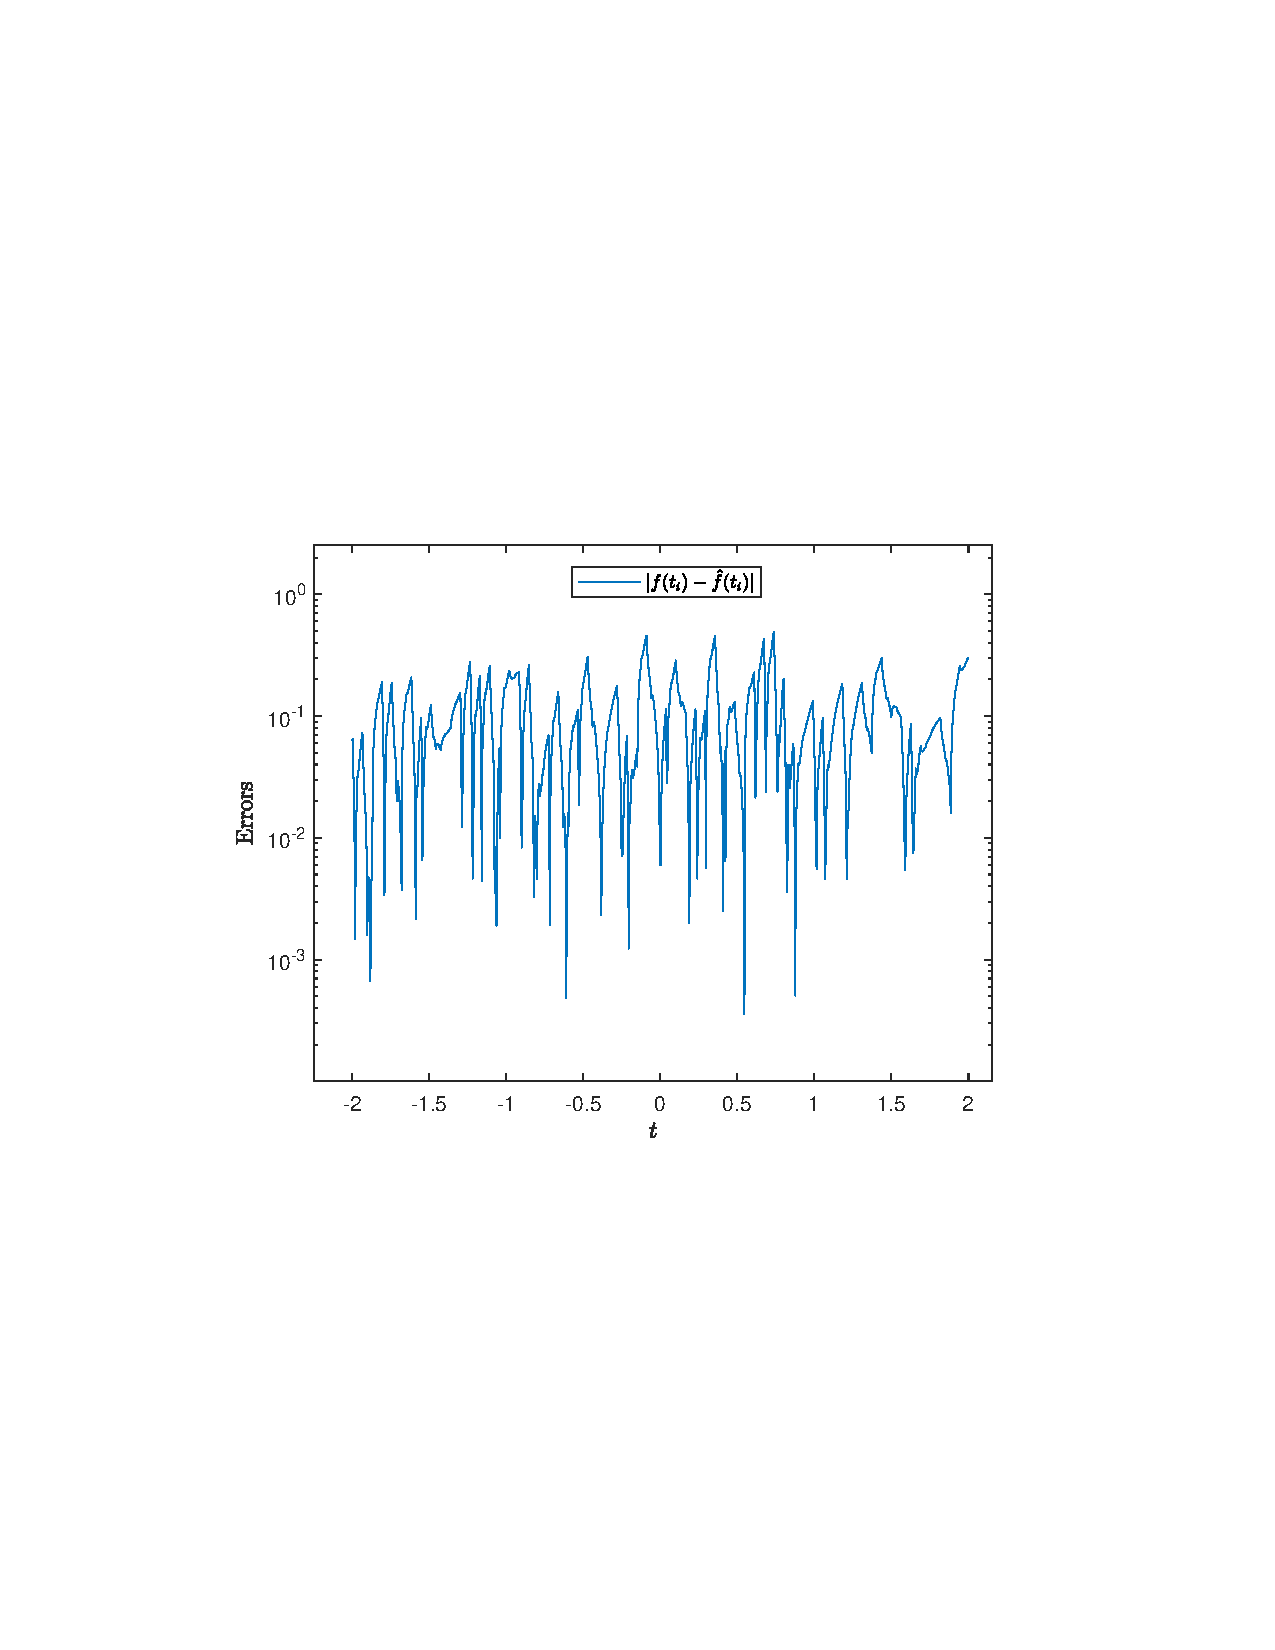
\includegraphics[trim={4cm 8cm 4cm 8cm},clip,width=1\textwidth]{Images/FuncRecStdError.pdf}
		\caption{The error between the clean function \cref{eq:func} and reconstructed ones}
		\label{sub:FuncRecStdError}
	\end{subfigure}
	\begin{subfigure}{0.49\textwidth}
		\centering
		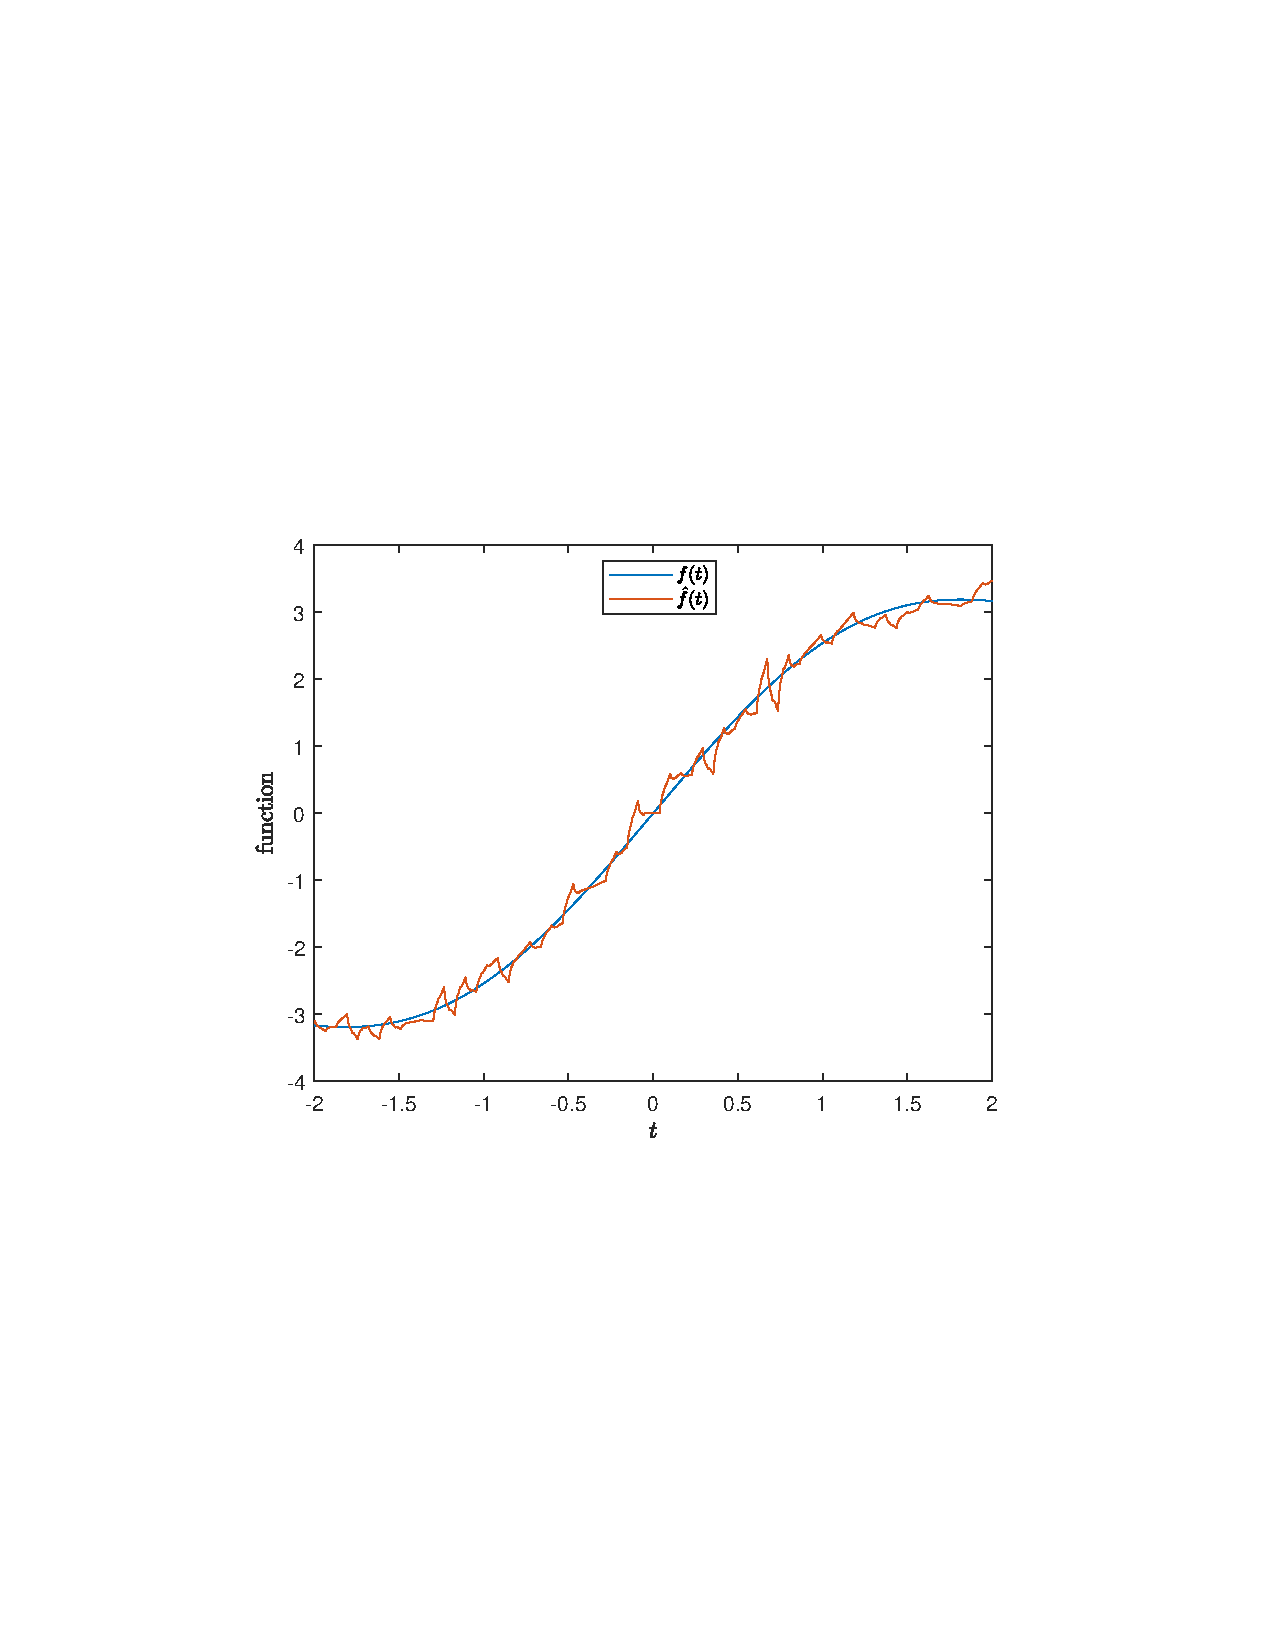
\includegraphics[trim={3.5cm 8cm 4cm 8cm},clip,width=1\textwidth]{Images/FuncRecStd.pdf}
		\caption{Plot of function \cref{eq:func} and reconstructed one}
		\label{sub:FuncRecStd}
	\end{subfigure}
	\caption{Plots for reconstruction of \cref{eq:funcNoise} via standard wavelet transform for wavelet \texttt{db2}, Level of decomposition 4, threshold of 1.73}
	\label{fig:FuncRecStd}
\end{figure}

	The best threshold for the redundant wavelet transform is 1.83, using hard thresholding. \texttt{SNR=12.801}. See \cref{fig:FuncRecRed} for results.
\begin{figure}[H]
	\centering
	\begin{subfigure}{0.49\textwidth}
		\centering
		%trim={<left> <lower> <right> <upper>}
		%\includegraphics[trim={4cm 8cm 4cm 8cm},clip,width=.49\textwidth]{Images/LQG_weighted4.pdf}
		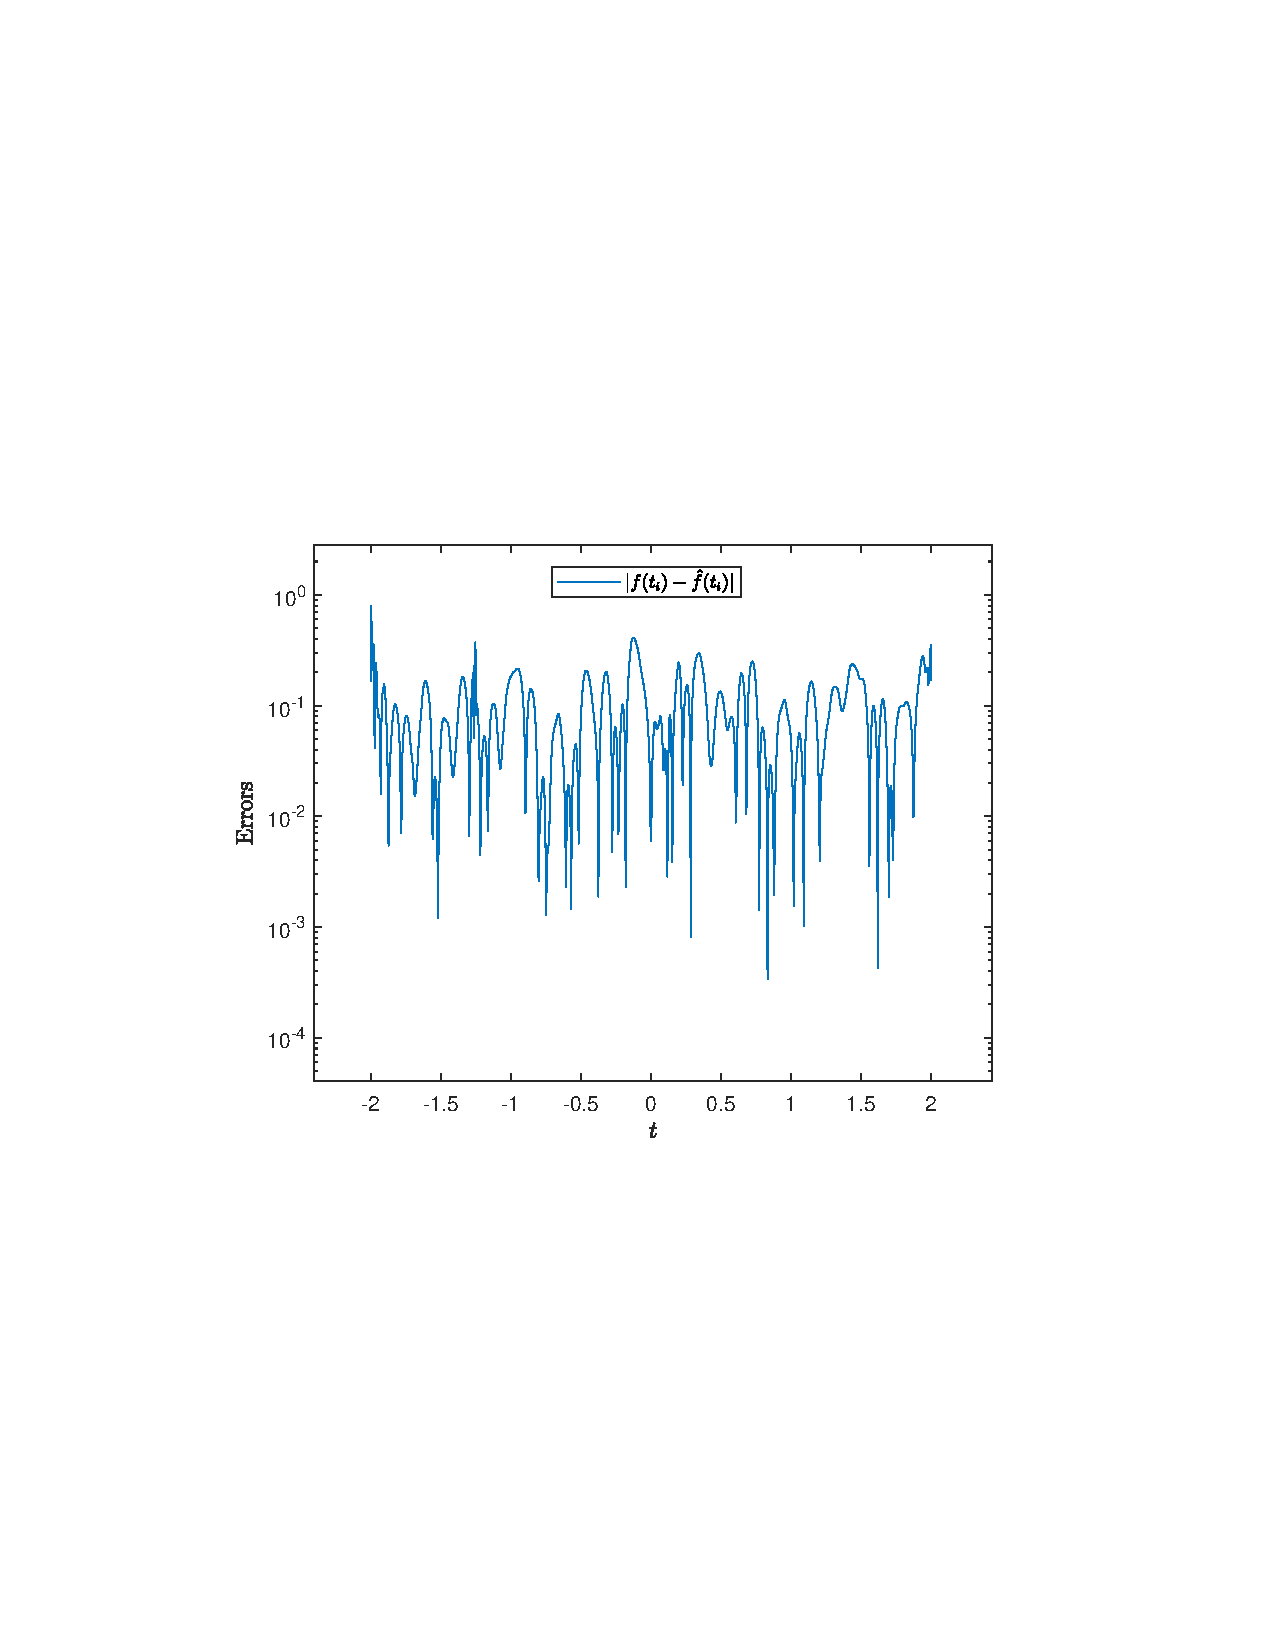
\includegraphics[trim={4cm 8cm 4cm 8cm},clip,width=1\textwidth]{Images/FuncRecRedError.pdf}
		\caption{The error between the clean function \cref{eq:func} and reconstructed ones}
		\label{sub:FuncRecStdRed}
	\end{subfigure}
	\begin{subfigure}{0.49\textwidth}
		\centering
		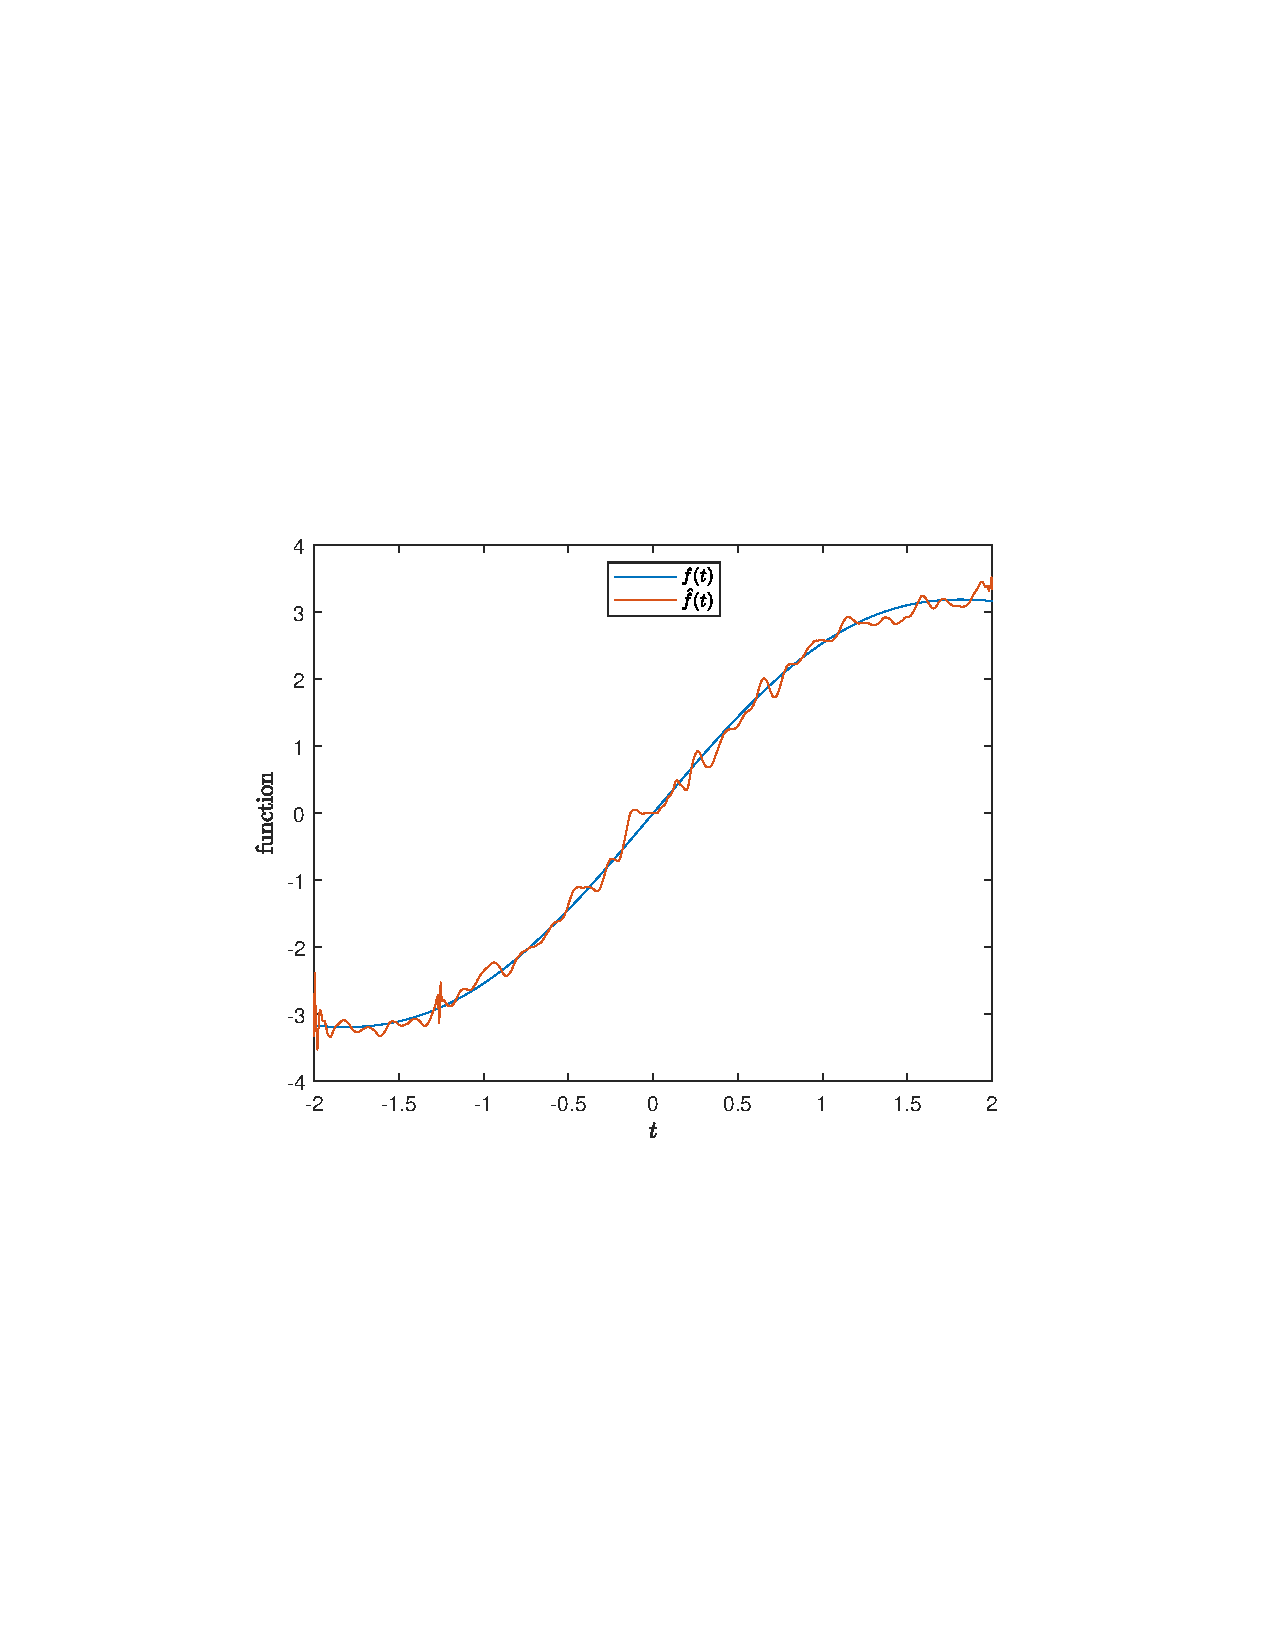
\includegraphics[trim={3.5cm 8cm 4cm 8cm},clip,width=1\textwidth]{Images/FuncRecRed.pdf}
		\caption{Plot of function \cref{eq:func} and reconstructed one}
		\label{sub:FuncRecRed}
	\end{subfigure}
	\caption{Plots for reconstruction of \cref{eq:funcNoise} via redundant wavelet transform for wavelet \texttt{db2}, Level of decomposition 4, threshold of 1.83}
	\label{fig:FuncRecRed}
\end{figure}

	We observe that reconstruction via redundant transform gives a smother function. And that \texttt{SNR} for redundant is higher then for standard, 12.801 vs 12.55. \\
	These results seem to point to the fact that redundant wavelet transform is better for denoising, this is to be expected since redundant transform does not do any downsampling, only upsampling.
	This means that unlike the standard wavelet transform which is critically sampled, the redundant transform has additional (redundant) information, which has the potential to have less loss of signal information during the thresholding.
    \subsubsection{Task 2.9}

	\newpage
	
    \section{Wavelet-based inpainting}

    \subsection{An iterative algorithm}

    \subsubsection{Task 3.1}

    \subsubsection{Question 3.2}

    \subsubsection{Question 3.3}

    \subsubsection{Question 3.4}

	\newpage

	\appendix
	
	\section{Tables}
	
	\begin{longtable}{| p{.20\textwidth} | p{.80\textwidth} |} 
	\hline
	foo & bar \\ \hline 
	foo & bar \\ \hline
	foo & bar \\ \hline
	foo & bar \\ \hline
	foo & bar \\ \hline
	foo & bar \\ \hline
	foo & bar \\ \hline
	foo & bar \\ \hline
	foo & bar \\ \hline
	foo & bar \\ \hline
	foo & bar \\ \hline
	\caption{Your caption here} % needs to go inside longtable environment
	\label{tab:myfirstlongtable}
\end{longtable}

	\section{Code}

 \end{document}